% =============================================================================
% Opposition Agents Playing Magic: The Gathering
% Knowledge-Graph-Grounded JEPA World Models and Active-Inference LLM Agents
%
% Tech report. Self-contained LaTeX (arXiv-compatible).
% Build:  pdflatex opposition_agents_mtg.tex
%         bibtex   opposition_agents_mtg
%         pdflatex opposition_agents_mtg.tex
%         pdflatex opposition_agents_mtg.tex
% =============================================================================
\documentclass[11pt,a4paper]{article}

\usepackage[utf8]{inputenc}
\usepackage[T1]{fontenc}
\usepackage{lmodern}
\usepackage[english]{babel}

\usepackage[margin=1in]{geometry}
\usepackage{microtype}
\usepackage{authblk}
\usepackage{amsmath, amssymb, amsthm}
\usepackage{mathtools}
\usepackage{graphicx}
\usepackage{booktabs}
\usepackage{multirow}
\usepackage{array}
\usepackage{tabularx}
\usepackage{enumitem}
\usepackage{xcolor}
\usepackage[authoryear,round]{natbib}
\usepackage[colorlinks=true,
            linkcolor=black,
            citecolor=blue!60!black,
            urlcolor=blue!60!black]{hyperref}
\usepackage{cleveref}
\usepackage{caption}
\usepackage{subcaption}
\usepackage{listings}
\usepackage{algorithm}
\usepackage{algpseudocode}
\usepackage{tikz}
\usetikzlibrary{shapes, arrows, arrows.meta, positioning, fit, backgrounds, calc}

% --- Theorems / definitions ---
\theoremstyle{definition}
\newtheorem{definition}{Definition}
\newtheorem{example}{Example}
\theoremstyle{plain}
\newtheorem{proposition}{Proposition}

% --- Notation ---
\DeclareMathOperator{\KL}{KL}
\DeclareMathOperator*{\argmin}{arg\,min}
\DeclareMathOperator*{\argmax}{arg\,max}
\DeclareMathOperator{\Expect}{\mathbb{E}}

% --- Listings (TOML / Cypher) ---
\definecolor{codebg}{RGB}{248,248,248}
\lstdefinelanguage{Cypher}{
  keywords={MATCH, RETURN, WHERE, CREATE, MERGE, WITH, OPTIONAL, AS, AND, OR,
           NOT, IN, EXISTS, LIMIT, ORDER, BY, DELETE, SET, REMOVE, CALL},
  sensitive=true,
  comment=[l]{//},
  string=[b]",
  morestring=[b]'
}
\lstset{
  basicstyle=\ttfamily\footnotesize,
  backgroundcolor=\color{codebg},
  frame=single,
  framerule=0pt,
  breaklines=true,
  showstringspaces=false,
  keywordstyle=\bfseries\color{blue!50!black},
  commentstyle=\color{green!30!black},
  stringstyle=\color{red!50!black},
  numbers=none
}

% =============================================================================
\title{\bfseries Neuro-Symbolic Agents Playing Magic: The Gathering\\[2pt]
       \large Ontology-Grounded Knowledge Graphs, Latent World Models,\\
       and Control-Theoretic Action Selection under Partial Observability}

\author[1]{Felix Neub\"urger}
\author[1]{Jonas Neub\"urger}
\affil[1]{Independent Research \\ \texttt{github.com/cuteredpwnda/opposition-agents-playing-mtg}}

\date{September 2026}

% =============================================================================
\begin{document}
\maketitle

\begin{abstract}
\noindent
\emph{Magic: The Gathering} (MTG) is, by several measures, the most combinatorially complex commercial card game ever published: more than 28{,}000 unique cards, a 260-page rule book, partial observability over 50--90 hidden cards, an unbounded action space, a turn-based stack with priority, and a state space conservatively estimated above $10^{800}$. We study agents that play it \emph{neuro-symbolically}: a verified rules engine decides what is legal, a formal ontology fixes what card semantics mean, a knowledge graph accumulates strategic structure, and learned components supply the statistics that no amount of symbolic knowledge can provide. Three claims organise the work. First, the symbolic layer should be a real ontology rather than a schema: we ground the agents in an OWL~2 DL ontology of MTG derived from the Comprehensive Rules and aligned to DOLCE, described separately \citep{neuburger2026ontology}. Second, the knowledge graph should be \emph{built by playing}: agents mine their own trajectories into an append-only, provenance-bearing extension layer that later agents query as a strategic prior, while curated card semantics remain untouched --- a population-level learning loop in which the graph is shared long-term memory rather than static context. Third, action selection should be posed as \emph{stochastic optimal control under partial observability} rather than as expected-free-energy minimisation: following \citet{kaufmann2026aifcontrol}, the canonical discretisation of Active Inference is belief-space KL control, so we implement that objective directly and retain the two conventional expected-free-energy factorisations only as ablation arms with documented failure modes. We describe the architecture, state where the symbolic/sub-symbolic boundary lies and what crosses it in each direction, and specify the evaluation that would test the control claim inside MTG rather than on toy POMDPs. Code, ontology, and traces are released under the MIT licence.
\end{abstract}

\vspace{0.5em}
\noindent\textbf{Keywords:} neuro-symbolic AI, knowledge graphs, world models, JEPA, stochastic optimal control, partially observable Markov decision processes, LLM agents, self-play, Magic: The Gathering.

% =============================================================================
\section{Introduction}
\label{sec:intro}

Reinforcement-learning (RL) research on games has historically progressed through a sequence of increasingly hard environments: backgammon \citep{tesauro1995temporal}, chess and Go \citep{silver2017mastering, silver2018alphazero}, StarCraft II \citep{vinyals2019grandmaster}, and no-limit Texas hold'em poker \citep{brown2018superhuman}. Each step pushed the community to invent new tools --- temporal-difference (TD) learning, deep value networks, self-play, counterfactual regret minimisation (CFR). \emph{Magic: The Gathering} (MTG) sits beyond the union of these challenges (\Cref{tab:complexity}): its action space is unbounded, its rules are open-textured natural language printed on cards (the comprehensive rule book itself defers to the per-card text in many places), its hidden information includes the entire opponent's deck composition, and its mechanics are extended every quarter by the publisher Wizards of the Coast. A single MTG card can override the rules of the game (e.g.\ \emph{Yixlid Jailer}, \emph{Blood Moon}, \emph{Cumulative Upkeep}), and a single decision in combat may resolve dozens of triggered abilities in a player-chosen order. The state space is open in the strict sense: every quarterly set adds previously-unseen card text whose semantics must be parsed at runtime, so any agent that hard-codes its action vocabulary cannot survive a set rotation.

For a concrete sense of why this matters for an algorithmic agent: in a single midgame turn the active player may need to (i) decide whether to play a land, (ii) sequence two or three spells with mana cost, colour requirements and stack ordering, (iii) optionally activate any number of permanent abilities that themselves go on the stack, (iv) declare attackers under summoning-sickness and tapping rules, (v) respond to triggered abilities resolving in the order chosen by their controllers, and (vi) decide which damage to assign in combat under multi-blocker rules. Each of these is itself a sub-decision tree. The total number of legal actions per priority pass routinely exceeds 60 and, in pathological combo states, several hundred. A model-free policy that emits a fixed-size logit vector cannot represent this branching, and a tabular search procedure that enumerates the subtree cannot fit it into memory.

\begin{table}[t]
\centering
\caption{Approximate combinatorial complexity comparison.}
\label{tab:complexity}
\small
\begin{tabularx}{\linewidth}{lXXXX}
\toprule
 & \textbf{Chess} & \textbf{Go} & \textbf{No-limit Poker (HU)} & \textbf{MTG} \\
\midrule
State space            & $10^{47}$  & $10^{170}$ & $10^{160}$ & $\boldsymbol{>10^{800}}$ \\
Branching factor       & $\sim$35   & $\sim$250  & $\sim$10   & $0$--$100^{+}$ (unbounded)\\
Hidden information     & none       & none       & 2 cards    & 50--90+ cards \\
Card / piece pool      & 6 types    & 1 type     & 52 cards   & $>$28{,}000 unique\\
Rule text length       & $\sim$10p  & $\sim$5p   & $\sim$10p  & $\sim$260p + per-card\\
Rules update frequency & decades    & decades    & decades    & quarterly \\
\bottomrule
\end{tabularx}
\end{table}

A purely model-free deep-RL approach is therefore unattractive: the action space cannot be enumerated as a fixed-size logit vector, the observation space is symbolic and irregular, and every new set introduces previously-unseen card text whose semantics must be parsed at run time. Conversely, a purely symbolic LLM-prompting approach struggles with rules-correctness, hallucinated cards, and the long-horizon credit-assignment that competitive play requires --- an LLM that simply names a move it would like to make has no guarantee that move is legal, that it resolves the way the LLM expects, or that it furthers a coherent multi-turn plan.

Our position is that the structure of MTG demands a \emph{neuro-symbolic} stack: a verified rules engine to keep play legal, a knowledge graph to make card semantics queryable, a learned world model to enable imagination and planning over the resulting compressed state, and an LLM agent that orchestrates these components under an active-inference objective. \Cref{fig:stack} sketches the resulting architecture as a data-flow diagram, separating the \emph{symbolic} substrate (data sources, engine, knowledge graph) from the \emph{learned} substrate (world model, agent zoo) and showing where information actually crosses the boundary.

\begin{figure*}[t]
\centering
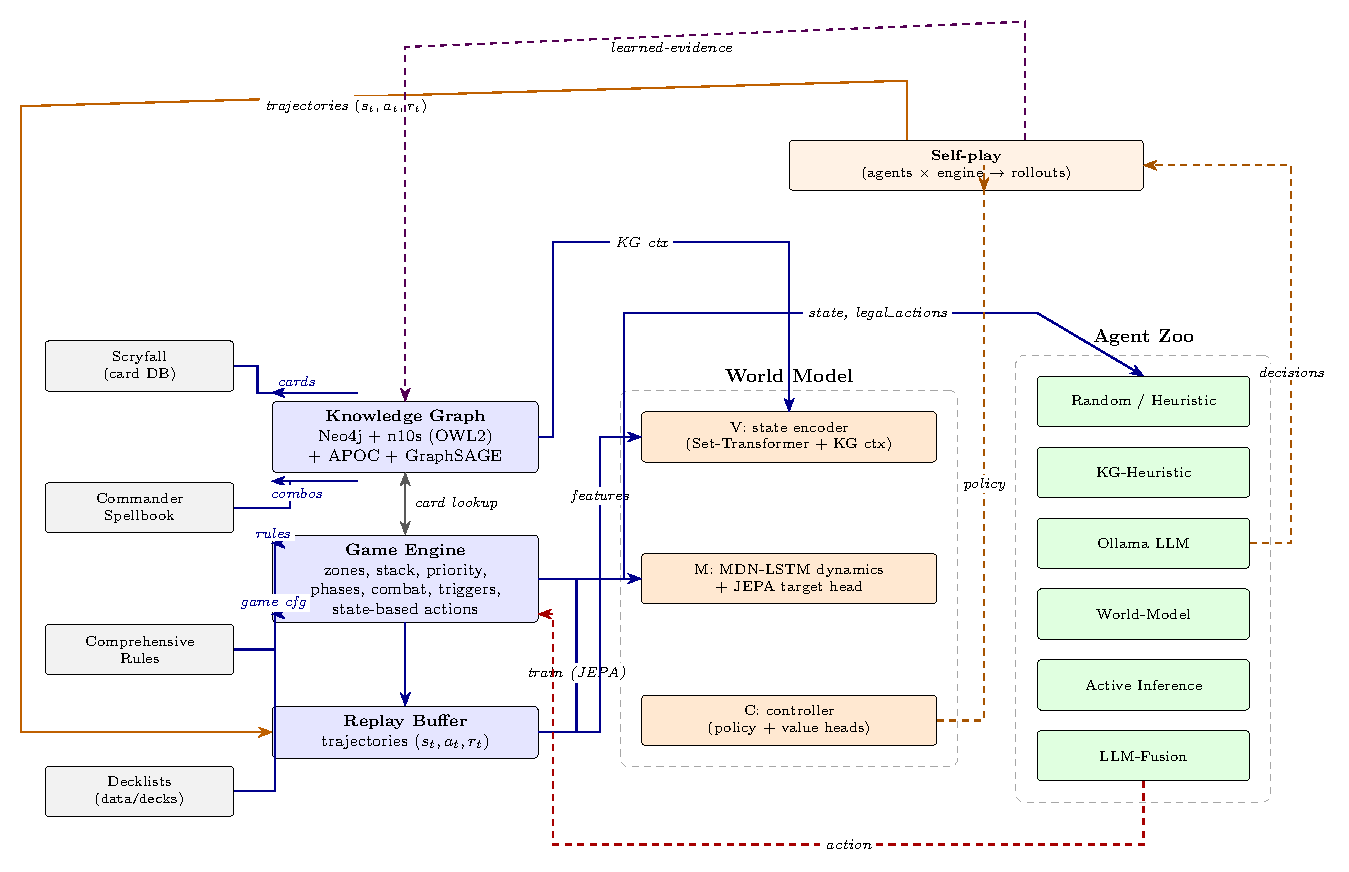
\includegraphics[width=\textwidth]{fig_stack.pdf}
\caption{Data-flow architecture. \textbf{Grey} boxes are external data sources; \textbf{blue} the symbolic substrate (engine, knowledge graph, replay buffer); \textbf{orange} the learned world model (V+M+C with a JEPA target head and a knowledge-graph context channel); \textbf{green} the agent zoo. Solid blue arrows are forward data flow; the red dashed arrow is the agent's chosen action returned to the engine; the engine $\leftrightarrow$ knowledge-graph link is bidirectional (card lookup at decision time, ontology-grounded card metadata at engine boot). Each agent additionally has read-only access to the knowledge graph and to the world-model controller through a thin lookup interface (omitted from the figure for clarity, described in the body text). The engine is the only component allowed to mutate game state; agents read but do not write.}
\label{fig:stack}
\end{figure*}

\paragraph{Contributions.} This work makes four contributions.
\begin{enumerate}[leftmargin=1.2em, itemsep=2pt]
  \item A scientific framing of MTG as an \emph{open-ended partially observable control problem} whose difficulty comes not only from combinatorics, but from the continual introduction of new symbolic rules through quarterly card releases.
  \item An architecture in which the symbolic/sub-symbolic boundary is stated rather than assumed (\Cref{sec:neurosymbolic}): what is symbolic, what is learned, what crosses in each direction, and what gates the crossing.
  \item A \emph{play-to-graph} learning loop in which agents mine their own trajectories into an append-only extension layer of the knowledge graph, and later agents query that layer as a strategic prior --- with curated card semantics protected from statistical contamination by construction (\Cref{sec:playtograph}).
  \item A \emph{control-theoretic} reading of MTG decision making: we adopt the result of \citet{kaufmann2026aifcontrol} that discrete Active Inference is belief-space KL control, implement that objective directly, and retain the two legacy expected-free-energy factorisations only as ablation arms (\Cref{sec:aif}).
\end{enumerate}

The ontology that grounds the symbolic layer is a contribution in its own right and is described in a companion paper \citep{neuburger2026ontology}; here we treat it as given and focus on what an agent does with it.

\paragraph{Why these four together.} Each contribution targets a specific failure mode of the others. The engine prevents the LLM from playing illegal moves and the world model from imagining inconsistent dynamics. The knowledge graph compresses the 28{,}000-card pool into a structure with a few hundred archetype clusters so that an agent can reason about ``what card type does this state want next'' without enumerating all candidates. The world model amortises the cost of multi-turn lookahead so that decisions remain well within a few hundred milliseconds even when planning ten turns deep. The active-inference fusion agent finally ties the three together with a single tunable objective --- expected free energy --- whose pragmatic and epistemic terms have a direct mapping onto MTG concepts of \emph{value} and \emph{information}.

\paragraph{Collective intelligence hypothesis.} Beyond single-agent optimisation, the same stack naturally supports a population-level learning loop: many heterogeneous agents generate trajectories, those trajectories are mined for repeated card-pair and outcome regularities, and the resulting evidence is written into an append-only graph extension layer with provenance. New agents then query this enriched graph and inherit strategic priors discovered by previous runs. In this reading, the KG is not only static symbolic context but a shared long-term memory for the entire agent population.

\paragraph{Scope and what we do \emph{not} do.} We do not solve MTG; we do not even target tournament-strength play. The contribution is a research substrate that is rules-correct on the implemented card pool, that maintains a queryable symbolic representation of card semantics, and that supports plug-in research on world models and inference-style agents on a problem qualitatively harder than the standard benchmarks. The empirical claims in \S\ref{sec:eval} are therefore framework-level (decks complete, agents converge faster than baselines, ablations show graded contributions) rather than absolute strength claims against human play.

The framework is released as open source\footnote{\url{https://github.com/cuteredpwnda/opposition-agents-playing-mtg}} and the codebase is the canonical artifact accompanying this report. Section~\ref{sec:related} positions the work against prior literature; \S\ref{sec:theory} formalises the POMDP and the four learning principles (world models, FEP, knowledge-graph priors, constrained-decoding LLMs); \S\ref{sec:arch} walks the architecture top-down; \S\ref{sec:eval} presents the empirical protocol and preliminary results; \S\ref{sec:limits}--\ref{sec:future} discuss limitations and next steps.

% =============================================================================
\section{Related Work}
\label{sec:related}

\paragraph{World models.} \citet{ha2018world} introduced the V+M+C decomposition --- a vision-VAE, a recurrent dynamics model with mixture-density output, and a tiny linear/MLP controller trained in the dream of M. Successors include Dreamer \citep{hafner2020dream, hafner2023dreamerv3} and the Schmidhuber-line of self-referential systems \citep{schmidhuber2015learning, irie2022neural}. We adopt the V+M+C skeleton but (i) replace the convolutional vision encoder with a Set-Transformer over symbolic game tokens, and (ii) attach a JEPA head \citep{lecun2022path, assran2023ijepa} that predicts a target encoding rather than a pixel-level reconstruction --- a closer fit to MTG, where ``imagination'' should preserve abstract game state, not card art. On the software side we now follow the modular research stack exemplified by \texttt{stable-pretraining}, \texttt{stable-worldmodel}, and LeWorldModel \citep{balestriero2025stable, maes_lelidec2026swm, maes_lelidec2026lewm}: the MTG-specific encoder, dynamics, and controller remain local to this repository, while stage-5 JEPA optimisation is delegated to the upstream training infrastructure.

\paragraph{Active inference and stochastic optimal control.} The Free-Energy Principle of \citet{friston2010free} and its discrete-state operationalisation \citep{sajid2021active} propose that action selection minimise \emph{expected free energy} (EFE), conventionally decomposed into a pragmatic (reward-seeking) and an epistemic (information-seeking) term. \citet{kaufmann2026aifcontrol} shows that this framing inverts the actual mathematical hierarchy: continuous-time Active Inference on path space \emph{is} finite-horizon path-integral stochastic MPC in the sense of \citet{kappen2005path}, \citet{todorov2009efficient} and \citet{williams2017mppi}, and its canonical discretisation is classical KL control on belief space. The exploration--exploitation trade-off is not supplied by an added epistemic term; it is Fel'dbaum's dual control effect \citep{feldbaum1960dual}, present in stochastic control from the outset, and it is recovered as soon as plans are evaluated \emph{closed-loop} over beliefs rather than as open-loop action sequences. We follow that result rather than the conventional decomposition, for the concrete engineering reasons set out in \Cref{sec:aif}: the two extant EFE factorisations have opposing, empirically demonstrated failure modes, and both are avoidable.

\paragraph{Knowledge graphs, GraphRAG, and their limits.} Neo4j with the \texttt{n10s} plugin enables direct ingestion of OWL ontologies as labeled property graphs \citep{neo4j_n10s}; the APOC library adds graph algorithms; GraphSAGE \citep{hamilton2017inductive} provides inductive node embeddings. GraphRAG \citep{edge2024graphrag} complements vector RAG for queries that benefit from explicit relational structure, and \citet{liao2026graphragbp} give the first component-level ablation of a GraphRAG pipeline, finding that retriever choice and graph \emph{serialisation format} dominate the outcome --- structured, code-like serialisations outperform prose renderings of the same subgraph. MTG is a textbook GraphRAG case: ``find me a two-card combo using only cards in my library that survive \emph{Counterspell}'' is a multi-hop graph query, not a similarity search. Two cautions from the same literature shape our design. \citet{diettrich2026harp} show that consumers of an evolving schema must discover it at runtime rather than assume it, because static pipelines fail silently under schema drift; and \citet{romanova2026relationships} gives a per-relation diagnostic for whether explicit graph structure still adds signal beyond node text at all, which is the honest way to decide where graph engineering is worth the effort.

\paragraph{Foundational ontologies and the symbolic layer.} The symbolic substrate of this system is an OWL~2~DL ontology of MTG aligned to DOLCE-UltraLite \citep{gangemi2002dolce, borgo2022dolce} and populated by mechanical derivation from the Comprehensive Rules. Its design, derivation pipeline and validation are the subject of a companion paper \citep{neuburger2026ontology} and are not restated here. What matters for the present argument is a property that most knowledge-graph-grounded agents lack: the vocabulary an agent reasons in is a checked artefact, in a decidable profile, with constraints stated as axioms rather than conventions. The broader turn toward competency-question-driven, validator-gated ontology construction \citep{garijo2026maseo, cq4oe2026, lippolis2026ontoextend, tiwari2026ontoprompt} is the methodological context for that work.

\paragraph{Neuro-symbolic systems and the curated/induced boundary.} The framing that organises \Cref{sec:neurosymbolic} is the distinction between \emph{curated} and \emph{induced} semantics. \citet{sabou2026neurosymbolic} argues that trustworthy neuro-symbolic AI requires explanations grounded in domain knowledge rather than saliency, and identifies provenance and continuous auditing as the missing infrastructure. \citet{thombre2026selfdemo} demonstrate that neuro-symbolic decomposition --- symbolic constraints narrowing the search space, the neural component reasoning inside each narrowed sub-task --- substantially outperforms monolithic prompting. \citet{vanschependom2026synthology} generate reasoning training data from an ontology by backward-chaining proof search, the natural route to a reasoning benchmark \emph{for} a schema such as ours. \citet{ehrenmuller2026sock} address the reconciliation of conflicting graph claims from heterogeneous sources with explicit methodological provenance, which is structurally the same problem as reconciling curated card semantics with statistics mined from imperfect self-play. Our contribution to this thread is a domain where the induced layer is generated by an agent acting in a \emph{verified} environment, so a learned assertion can in principle be traced back to the exact game states that support it.

\paragraph{MTG and other complex card games.} Earlier MTG-AI work has used hand-crafted heuristics \citep{cowling2012ensemble}, MCTS, and small policy nets on restricted card pools (e.g., \texttt{open-mtg}). On the rules side, \texttt{Forge}, \texttt{XMage} and \texttt{Mage} provide JVM-based reference implementations, and \texttt{phase-rs} provides a Rust one. To our knowledge, no prior public system combines a full Comprehensive-Rules engine with a learned world model and a foundational-ontology-grounded symbolic layer. \citet{moravvcik2017deepstack} (poker), \citet{vinyals2019grandmaster} (StarCraft) and \citet{schrittwieser2020mastering} (MuZero) are spiritual antecedents at the algorithmic level.

\paragraph{Ontologies for games.} Game ontologies have been explored for serious games and educational metadata; for trading-card games specifically, public OWL ontologies are sparse and, where they exist, are unaligned flat vocabularies. The ontology used here \citep{neuburger2026ontology} is, to our knowledge, the first for a trading card game that is both in the OWL~2~DL profile and foundationally aligned.

% =============================================================================
\section{Theoretical Foundations}
\label{sec:theory}

\subsection{MTG as a partially-observable Markov game}
We model a game of Magic from the perspective of a single seat as a finite-horizon POMDP $(\mathcal{S}, \mathcal{A}, \mathcal{O}, T, \Omega, R, \gamma, b_0)$ embedded inside an $n$-player Markov game.  The full state $s_t \in \mathcal{S}$ encompasses every public and private zone of every player --- libraries, hands, the stack, mana pools, and a long tail of bookkeeping flags (summoning sickness, monarchy, the day/night state, designations, emblems, dungeon room, companion eligibility).  A controlled-perspective filter $\Omega: \mathcal{S} \to \mathcal{O}$ hides the opposing players' hands and the order of their libraries; the agent only ever observes $o_t = \Omega(s_t)$.  The action space $\mathcal{A}_t = \mathrm{LEGAL}(s_t)$ is computed afresh on every priority pass and is highly variable: typically $|\mathcal{A}_t| \in [1, 60]$, but can spike past several hundred in hard combo states.  The transition model $T(s' \mid s, a)$ is the rules engine itself, fully deterministic given a random seed and the active player's choices.  Reward $R$ is sparse and terminal --- $\pm 1$ on the win condition --- but agents may shape it during training using $\Delta\text{life}$, $\Delta\text{cards}$, $\Delta\text{tempo}$ as auxiliary signals.  The state space is combinatorially large: a conservative count over deck-times-zone configurations gives $|\mathcal{S}| > 10^{800}$, several orders of magnitude beyond Go.

The optimal value function over beliefs $b_t \in \Delta(\mathcal{S})$ satisfies the Bellman equation
\begin{equation}
V^*(b) = \max_{a \in \mathcal{A}} \left[ \sum_s b(s)\, R(s,a)
   + \gamma \sum_o \Pr(o \mid b, a) \, V^*\!\big(b'_o\big) \right],
\end{equation}
where $b'_o$ is the Bayes update of $b$ after taking $a$ and observing $o$.  Exact solution is intractable.  Each agent in our zoo is therefore an explicit approximation that trades different axes of accuracy: tabular reactive policies (Random, Heuristic, KG-Heuristic, LLM) collapse $b_t$ to a point estimate $s_t \approx o_t$; the world-model agent learns an amortised Bellman residual in latent space; the active-inference agents maintain an explicit belief and minimise expected free energy.

\subsection{World models as latent imagination}
The V+M+C decomposition of \citet{ha2018world} factors an agent into a perception module $V$, a recurrent dynamics module $M$, and a controller $C$.  We follow this skeleton but adopt LeCun and Assran's recommendation \citep{lecun2022path, assran2023ijepa} to predict in \emph{representation space} rather than in observation space: the model is trained to match its $H$-step rollout of the latent against a target encoder's output, not to reconstruct cards or board art.  Concretely the training loss for the dynamics is
\begin{equation}
\mathcal{L}_{\text{JEPA}}
= \sum_t \big\| \hat z_{t+1} - \mathrm{sg}(z_{t+1}) \big\|^2_2
  \,+\, \beta \cdot \mathrm{KL}\!\left( q(z_t \mid o_t) \,\big\|\, p(z_t \mid h_{t-1}) \right),
\label{eq:jepa-loss}
\end{equation}
where $\mathrm{sg}$ is stop-gradient on the target branch, $h_{t-1}$ is the previous LSTM hidden state of $M$, and $\beta$ is the single tunable hyperparameter we expose (\texttt{--jepa-beta}, default 1.0).  At decision time the controller scores each candidate action by a $K{\times}H$ Monte-Carlo rollout in latent space:
\begin{equation}
\mathrm{score}(a) = \frac{1}{K} \sum_{k=1}^{K} V_\theta\!\left( h^{(k)}_{t+H} \,\big|\, a_t = a \right),
\label{eq:wm-rollout}
\end{equation}
with $K = 8$, $H = 10$ by default.  No actual rules-engine simulation is performed during inference; this is what makes the agent fast despite the engine being heavy.  The controller therefore amortises the Bellman residual: $C$ is implicitly approximating $\arg\max_a Q^*(s_t, a)$ given an imperfect $\hat T$.

\paragraph{Training implementation note.} The current stage-5 training path keeps the MTG architecture in \texttt{src/world\_model/world\_model.py} but wraps optimisation in \texttt{stable\_pretraining.Manager} and Lightning callbacks rather than a bespoke trainer. We keep \texttt{stable-worldmodel} in the stack as the upstream world-model research substrate and benchmark interface, matching the layering used by LeWorldModel \citep{maes_lelidec2026swm, balestriero2025stable, maes_lelidec2026lewm} while preserving MTG-specific state encoding, graph fusion, and legal-action masking locally.

\subsection{Active inference as path-integral control}
\label{sec:aif}

Friston's free-energy principle \citep{friston2010free} frames perception and action as two sides of variational inference under a generative model $p(o,s)$. Variational free energy decomposes as
\begin{equation}
F[q] = \mathbb{E}_q[\log q(s) - \log p(o,s)] = \mathrm{KL}\!\big(q(s) \,\|\, p(s \mid o)\big) - \log p(o),
\end{equation}
so minimising $F$ over $q$ simultaneously sharpens beliefs and accumulates evidence. Action selection is then conventionally recovered by minimising \emph{expected} free energy. It is at this second step that the literature fractures, and where we depart from it.

\paragraph{The path-space objective.} Following \citet{kaufmann2026aifcontrol}, write the agent's goals as a preference prior $p(\eta)$ over \emph{latent plant state} $\eta$ --- the state of the game itself --- and define the potential
\begin{equation}
V(\eta) := -\log p(\eta).
\label{eq:potential}
\end{equation}
Let $Q^{u}$ be the path measure induced on a planning horizon by control $u$, and let $P_0$ be the uncontrolled (passive) path measure. The Gibbs tilt $P_V \propto e^{-V(\eta_T)} P_0$ is the target. Path-form expected free energy is then simply the relative entropy of the controlled path measure against the target,
\begin{equation}
G[u] \;=\; \mathrm{KL}\!\big(Q^{u} \,\big\|\, P_V\big),
\label{eq:pathefe}
\end{equation}
and by Girsanov's theorem this equals, up to policy-independent constants, a finite-horizon stochastic MPC objective with quadratic control cost and terminal potential $V$. Minimising expected free energy \emph{is} path-integral control.

\paragraph{The discrete counterpart we implement.} Time-slicing \eqref{eq:pathefe} gives belief-space KL control:
\begin{equation}
G(\pi) \;=\; \underbrace{\mathrm{KL}\!\big(Q(\eta \mid \pi) \,\big\|\, P_0(\eta)\big)}_{\text{control cost } C_{\mathrm{action}}}
          \;+\; \underbrace{\mathbb{E}_{Q(\eta \mid \pi)}\!\big[V(\eta)\big]}_{\text{risk}}.
\label{eq:klcontrol}
\end{equation}
Two things are absent from \eqref{eq:klcontrol} and their absence is deliberate. There is \textbf{no additive information-gain bonus} and there is \textbf{no ambiguity (likelihood-entropy) penalty}. Measurement likelihoods belong to the observation filtration that drives the belief estimator; they are not part of the plant objective. Exploration is recovered instead from Fel'dbaum's dual control effect \citep{feldbaum1960dual}: because $\pi$ is evaluated \emph{closed-loop} over belief states with observation branching, an action that sharpens the posterior unlocks cheaper continuations and therefore lowers $\mathbb{E}[V(\eta_T)]$ on its own. A probe is taken if and only if the resulting drop in expected terminal potential exceeds its control cost --- which is exactly the condition one wants, and which no hand-tuned coefficient has to encode.

\paragraph{Why not the conventional factorisations.} The two EFE forms in common use are
\begin{align}
G_{\mathrm{IG}}(\pi) &= - \underbrace{\mathbb{E}_{Q}\!\big[\log Q(\eta \mid s) - \log Q(\eta)\big]}_{\text{information gain}} - \underbrace{\mathbb{E}_{Q}\!\big[\log p(s)\big]}_{\text{pragmatic}}, \label{eq:efe1}\\
G_{\mathrm{AMB}}(\pi) &= \underbrace{\mathrm{KL}\!\big(Q(\eta\mid\pi)\,\|\,\tilde p(\eta)\big)}_{\text{risk}} + \underbrace{\mathbb{E}_{Q}\!\big[\mathrm{H}[p(s \mid \eta)]\big]}_{\text{ambiguity}}, \label{eq:efe2}
\end{align}
and they are known to coincide only when the sensory preference $p(s)$ is exactly the pushforward of the state preference through the observation channel \citep{millidge2021whence} --- a condition hand-authored preferences essentially never satisfy. Each also has a characteristic pathology, and both have a concrete MTG shape:

\begin{itemize}[leftmargin=1.2em, itemsep=2pt]
  \item \eqref{eq:efe1} rewards information for its own sake and is captured by \emph{noisy-TV} distractors. In MTG this manifests as compulsive scry/surveil/cantrip loops: the agent repeatedly buys information about the top of its library because the bonus is unconditional, while the board state deteriorates.
  \item \eqref{eq:efe2} penalises outcome entropy and induces \emph{scotophobia}. In MTG this manifests as refusal to attack into possible blockers or to cast into open mana --- lines whose variance is high but whose expectation is strictly favourable.
\end{itemize}

Both are implemented in \texttt{src/agents/kl\_control.py::LegacyEFE} purely so that \Cref{sec:eval-aif-ablation} can measure these failure modes in our domain rather than assume them.

\paragraph{Bounded rationality.} Deliberation is not free. Under a finite cognitive budget the hard $\min$ is replaced by the softmin (free-energy) operator and policy selection follows the bounded-optimal Gibbs distribution
\begin{equation}
p_\beta(\pi) \;=\; \frac{1}{Z_\beta}\, q(\pi)\, e^{-\beta\, G(\pi)},
\qquad
\operatorname{softmin}_\beta(x) = -\tfrac{1}{\beta}\log \textstyle\sum_i q_i e^{-\beta x_i},
\label{eq:gibbs}
\end{equation}
which recovers the deterministic Bellman minimiser as $\beta \to \infty$ and the passive prior as $\beta \to 0$. A single scalar $\beta$ therefore interpolates between a greedy planner and a prior-following one, and it has an operational meaning (how much compute we are willing to spend per priority window) rather than being a free knob.

\paragraph{Where the other signals go.} The passive prior $q$ in \eqref{eq:klcontrol}--\eqref{eq:gibbs} is load-bearing. It is the reference measure the control cost is charged against, which gives the heuristic, knowledge-graph and language-model signals a principled home: they \emph{shape} $q$, and deviating from the resulting informed default carries a thermodynamic price $-\log q(a)$. In the previous version of this system those three signals entered as an additive weighted sum with hand-set coefficients $(\alpha_h,\alpha_g,\alpha_w,\alpha_\ell)$; \eqref{eq:klcontrol} replaces that with a single objective in which their role is determined rather than chosen.

\subsection{Knowledge graphs as a symbolic prior}
Cards form an inductive graph $\mathcal{G} = (V, E, \tau)$ with typed edges $\tau \in \{\text{combo}, \text{synergy}, \text{counter}, \text{enables}\}$ ingested from the OWL ontology and an embedding pipeline trained with GraphSAGE \citep{hamilton2017inductive}.  GraphSAGE is inductive: a freshly printed card $v_{\text{new}}$ obtains an embedding $\mathbf{h}_{v_{\text{new}}} \in \mathbb{R}^{128}$ by sampling and aggregating its neighbours, without retraining.  We exploit this in two ways: (i) the encoder feeds a graph latent $g_t = \mathrm{Enc}_{KG}(\mathcal{G}, s_t)$ into the recurrent dynamics so that the world model's prior is graph-aware, and (ii) the passive prior $q$ of \eqref{eq:klcontrol} is tilted by graph distance to combo completions, mirroring GraphRAG's ``relational evidence'' pattern \citep{edge2024graphrag}.

In implementation, we separate immutable source facts (card oracle data, ontology-grounded edges) from learned extension evidence. Self-play enrichment appends provenance-linked learned nodes/edges instead of mutating base facts, allowing many agents and runs to contribute to one shared strategic memory while preserving reproducibility and auditability. \Cref{sec:ontology} makes this separation a property of the schema rather than a convention.

\subsection{The neuro-symbolic boundary}
\label{sec:neurosymbolic}

``Neuro-symbolic'' is used loosely enough that it is worth stating exactly what is symbolic here, what is learned, and what crosses between them. The system contains three symbolic artefacts and three learned ones, and the interfaces between them are narrow by construction.

\paragraph{Symbolic side.} (i) The \texttt{phase-rs} rules engine is a verified, deterministic transition system: it decides legality, resolves the stack, applies state-based actions, and is the only component permitted to mutate game state. (ii) The OWL~2~DL ontology (\Cref{sec:ontology}) fixes the vocabulary in which card semantics, turn structure, roles, and strategic constructs are expressed, and is checked by a reasoner and by SHACL shapes. (iii) The knowledge graph is the ABox populated against that TBox from Scryfall and combo databases.

\paragraph{Learned side.} (i) A GraphSAGE encoder turns the graph into dense node embeddings. (ii) The JEPA world model learns latent dynamics from self-play trajectories. (iii) Language models supply a prior over the legal-action set.

\paragraph{What crosses, and in which direction.} The crossings are the substance of the architecture:

\begin{enumerate}[leftmargin=1.4em, itemsep=2pt]
  \item \textbf{Symbolic $\rightarrow$ neural (structure as inductive bias).} Graph structure is compiled into the encoder's context channel $g_t$, and the legal-action set produced by the engine masks the controller's output. The neural components therefore never have to learn legality or card identity; they learn only what is genuinely statistical.
  \item \textbf{Symbolic $\rightarrow$ neural (structure as reference measure).} The knowledge graph and the heuristic shape the passive prior $q$ of \eqref{eq:klcontrol}. Symbolic knowledge thus enters the control objective as a \emph{cost of deviation}, not as an additive score.
  \item \textbf{Neural $\rightarrow$ symbolic (induction of new relations).} Self-play traces are mined into candidate relations --- card co-occurrence in winning positions, answer/threat pairs, archetype signatures --- and written back as \emph{induced} assertions. This is the direction most neuro-symbolic systems leave empty, and it is where the interesting failure modes live: a statistical regularity is not an ontological commitment.
  \item \textbf{Validation as the gate between them.} Nothing induced is promoted to curated status automatically. Candidate relations are reified, weighted, attributed to the run that produced them, and validated by the shapes and reasoner before a human may accept them. This mirrors the finding of \citet{tiwari2026ontoprompt} that the validator, not the generator, is what turns diverse neural proposals into a high-precision graph.
\end{enumerate}

\paragraph{Curated versus induced semantics.} The design commitment underlying all four crossings is that deterministic facts and learned regularities must remain distinguishable forever. A card's oracle text is curated: it is definitional, immutable, and wrong is wrong. That two cards co-occur in 83\,\% of the games one of them wins is induced: it is defeasible, provenance-bearing, and may be an artefact of the deck pool sampled. Collapsing the two --- writing a learned edge into the same relation as a curated one --- destroys the ability to recover ground truth and makes the graph unauditable. \Cref{sec:ontology} enforces the distinction with an \texttt{mtg:epistemicStatus} annotation on every axiom and a schema-level requirement that no induced assertion may exist without a \texttt{prov:Activity} that generated it.

\subsection{LLM as a constrained-decoding policy}
The LLM never freely generates moves.  Given the prompt $\rho(s_t, \mathcal{A})$ that enumerates legal actions by index, we read off
\begin{equation}
\log p_{\text{LLM}}(a \mid s_t) = \mathrm{LM}\!\big( \mathrm{idx}(a) \,\big|\, \rho(s_t, \mathcal{A}) \big),
\end{equation}
masking any token outside the integer range $\{0, \dots, |\mathcal{A}|-1\}$.  This recovers the standard ``constrained decoding'' guarantee --- the LLM cannot hallucinate an illegal move --- while still letting it import its general-knowledge prior.  Calibration of the resulting distribution is controlled by a temperature parameter ($0.2$ in our default config), which interpolates between greedy LLM picks and a uniform fallback.

\subsection{Self-play promotion as fixed-point iteration}
Training combines all three signals.  The replay buffer $\mathcal{D}$ is collected by self-play between agent variants; the world model is fit on $\mathcal{D}$; and the controller is improved iteratively by the champion-vs-challenger schema implemented in \texttt{scripts/train\_pipeline.py}.  At each iteration $i$, a challenger $\pi_{i+1}$ is trained against $\pi_i$ on the latest replay window and faces the champion in a best-of-$N$ match; promotion happens iff the empirical win rate exceeds $0.55$.  This is a stochastic-approximation fixed-point operator on the policy improvement step \citep{tesauro1995temporal, silver2017mastering, silver2018alphazero, schrittwieser2020mastering}: under standard Robbins--Monro conditions it converges, in expectation, to a fixed point of the Bellman optimality operator restricted to the dynamics class $\hat T$ that the world model has learned.  Convergence in practice depends on $\hat T$ being locally accurate, which we monitor by tracking JEPA validation loss across iterations.

% =============================================================================
\section{System Architecture}
\label{sec:arch}

\subsection{Game engine}
The runtime engine is \texttt{phase-rs} (Rust), accessed over its
WebSocket interface via \texttt{src/integrations/phase\_rs/}.
Our Python side is intentionally adapter-only at execution time:
\texttt{client.py} handles protocol envelopes,
\texttt{runner.py} drives game loops,
\texttt{adapter.py} maps legal actions/snapshots into our policy API,
and \texttt{server\_process.py} manages local server lifecycle for
training scripts.

\paragraph{Tracking a living upstream.} \texttt{phase-rs} is under active
development and its wire protocol is versioned and enforced at handshake.
Over the period covered by this report the upstream protocol advanced from
v6 to v75, which is a useful reminder that an external rules engine is a
dependency with its own release cadence, not a fixed substrate. Two of
those changes were structural rather than additive and required adapter
work: rejections became a typed \texttt{ActionRejection} carrying a stable
machine-readable code and a recovery disposition rather than a prose
string, and the engine now publishes \emph{viewer interactions} --- an
explicit, engine-authored protocol for the choices a player must make
during resolution (targets, modes, damage assignment, ordering). The
second is the more significant for us: it moves a large class of
decisions out of the flat \texttt{legal\_actions} list into a structured
opportunity schema, which is strictly better for an agent that wants to
reason about \emph{what kind} of choice it is making. We pin the protocol
constant in \texttt{client.py} and fail closed on mismatch rather than
attempting to negotiate, on the principle that a silently
misinterpreted game state is worse than a refused connection.

Core integration modules:
\begin{itemize}[leftmargin=1.2em, itemsep=1pt]
  \item \texttt{client.py}: protocol handshake, message parsing, and typed
    message dataclasses for \texttt{GameStarted}, \texttt{StateUpdate},
    and \texttt{GameOver};
  \item \texttt{runner.py}: end-to-end game loop for a Python-controlled seat,
    including structured per-decision JSONL traces;
  \item \texttt{adapter.py}: practical \texttt{GameAction} $\leftrightarrow$
    \texttt{Action} bridge and snapshot projection for native Python
    policies;
  \item \texttt{agent\_bridge.py}: random/heuristic/LLM pickers plus
    adapter-backed native-agent picker support;
  \item \texttt{server\_process.py}: managed local \texttt{phase-server}
    process startup/shutdown for reproducible training/evaluation runs.
\end{itemize}
The old Python engine remains in-repository as legacy compatibility code,
but new experiments and reported benchmarks use \texttt{phase-rs} as the
authoritative runtime transition system.

\Cref{tab:engine-pointers} maps each Comprehensive-Rules concept to the exact module that implements it; readers reproducing the system can use it as a reading order through the codebase.

\begin{table}[t]
\centering
\small
\setlength{\tabcolsep}{4pt}
\renewcommand{\arraystretch}{1.05}
\begin{tabular}{@{}p{0.40\textwidth} p{0.18\textwidth} p{0.36\textwidth}@{}}
\toprule
\textbf{Comprehensive Rules concept} & \textbf{CR section} & \textbf{Implementing module} \\
\midrule
Turn structure / phases / steps          & 500--514         & \texttt{src/engine/phases.py} \\
APNAP priority \& priority loop          & 116--117         & \texttt{src/engine/priority\_loop.py} \\
The stack \& spell resolution            & 405--608         & \texttt{src/engine/stack.py} \\
Layer system (continuous effects)        & 613              & \texttt{src/engine/continuous\_effects.py} \\
Replacement effects                      & 614--616         & \texttt{src/engine/replacement\_effects.py} \\
Triggered abilities                      & 603              & \texttt{src/engine/triggered\_abilities.py} \\
State-based actions                      & 704              & \texttt{src/engine/state\_based\_actions.py} \\
Combat (declare, block, damage steps)    & 506--510         & \texttt{src/engine/combat.py} \\
Mana \& cost payment                     & 106, 601--602    & \texttt{src/engine/mana.py} \\
London mulligan                          & 103.5            & \texttt{src/engine/game\_setup.py} \\
Cleanup discard to hand size             & 514              & \texttt{src/engine/phases.py::cleanup\_step} \\
Loss from empty library on draw          & 104.3c, 704.5b   & \texttt{src/engine/state\_based\_actions.py} \\
Legal-action enumeration                 & --- (engine-internal) & \texttt{src/engine/rules\_engine.py} \\
\bottomrule
\end{tabular}
\caption{Mapping from Comprehensive-Rules concepts to the implementing engine module. Every cell is a real path; auditing a rule reduces to opening that file. The legal-action enumerator (\texttt{rules\_engine.py}) is the only point of contact between the engine and any agent.}
\label{tab:engine-pointers}
\end{table}

\subsection{Symbolic substrate: the ontology}
\label{sec:ontology}

The symbolic layer is an OWL~2~DL ontology of MTG derived from the Comprehensive Rules and aligned to the DOLCE-UltraLite foundational ontology. It is a contribution in its own right and is described in a companion paper \citep{neuburger2026ontology}; we summarise here only what an agent actually depends on.

Three properties matter for the argument of this paper. First, the ontology is \emph{expressive enough to be wrong}: it is in the DL profile, so a reasoner can be run against it, and constraints such as the card-type/subtype correlation of CR 205.3 are stated as axioms rather than left as prose. An agent querying it is querying something that has been checked. Second, its content is \emph{derived, not curated by hand}: 3{,}161 rules and roughly 550 type and keyword individuals are generated from the rules text, each grounded in the rule that licenses it, so the vocabulary tracks the game as the publisher extends it. Third, and most importantly here, it distinguishes \emph{curated} from \emph{induced} assertions at the schema level. That distinction is what makes the learning loop of \Cref{sec:playtograph} safe.

For orientation: cards are imported from Scryfall as \texttt{CardDesign} nodes with oracle text and an SBERT embedding; mechanics, abilities, archetypes and combos are first-class nodes; APOC supplies PageRank, community detection and shortest-path queries; and multi-hop retrieval over this structure is the ``relational evidence'' pattern of GraphRAG \citep{edge2024graphrag}, which suits questions --- \emph{which two cards in my library combo, and does either die to a counterspell?} --- that similarity search answers badly.

\subsection{Playing to build the graph}
\label{sec:playtograph}

The knowledge graph is usually treated as a fixed input: someone curates it, the agent reads it. We are interested in the other direction as well, because an agent that plays thousands of games observes something a curator cannot --- which cards actually co-occur in positions that get won, against which opponents, at which points on the curve.

The loop has four steps. Agents play on the rules engine and emit structured decision traces. Traces are post-processed into candidate relations: card pairs recurring in winning positions, answer/threat pairs, archetype signatures. Candidates are written into the graph as \emph{induced} assertions --- reified, weighted by support and refutation counts, and attributed under PROV-O to the run that produced them. Later agents query those assertions as an additional prior, and their play produces the next round of evidence.

Two design commitments keep this from degenerating.

\paragraph{The extension layer is append-only and typed apart.} An induced synergy is not an edge in the curated \texttt{synergisesWith} relation; it is a reified evidence node that the schema requires to be attributable to an activity. A consumer needing deterministic ground truth recovers it by filtering on epistemic status. This matters because the two kinds of claim have different logic: a card's oracle text is definitional and wrong is wrong, whereas a co-occurrence statistic is defeasible and may be an artefact of the deck pool sampled. Systems that write learned edges into curated relations lose the ability to tell the difference, and with it the ability to audit.

\paragraph{Promotion is not automatic.} Nothing is reclassified from induced to curated without a human. We regard the promotion gate --- what support threshold, what handling of disagreement between runs \citep{ehrenmuller2026sock} --- as an open problem rather than a solved one, and say so in \Cref{sec:limits}.

\paragraph{Agent reasoning is itself in the graph.} A decision is recorded as a \texttt{prov:Activity} carrying the objective decomposition it was selected by, the belief it was taken under, and the policy precision in force. ``Why did seat~0 attack on turn~6?'' is therefore a graph query rather than a log grep. This is a deliberate response to the observation \citep{sabou2026neurosymbolic} that trustworthy neuro-symbolic systems need explanations grounded in domain knowledge with provenance attached, rather than post-hoc attribution scores; it also means the explanation and the game state it refers to are expressed in one vocabulary.

\paragraph{Collective intelligence, stated carefully.} The attractive reading is that heterogeneous agents accumulate shared strategic memory across runs, so that later agents inherit what earlier ones discovered without retraining. The framework supports that reading structurally. We have not yet demonstrated it: showing that graph enrichment from run $n$ measurably improves agents in run $n{+}1$, and is not merely overfitting to a fixed deck pool, is the experiment that would substantiate the claim, and it is not among the results reported here.

\subsection{World model}
\label{sec:wm}
Let $s_t \in \mathcal{S}$ be the game state at decision step $t$ and $g \in \mathcal{G}$ the player's KG context (deck, archetype tag, known opponent information). The world model decomposes as:
\begin{align}
z_t       &= \mathrm{Enc}_V(s_t)            && \text{(state encoder, Set-Transformer + VAE)} \\
g_t       &= \mathrm{Enc}_{\mathrm{KG}}(g, s_t) && \text{(KG context encoder)} \\
h_t, \pi^M_t &= \mathrm{LSTM}_M\!\big([z_t; g_t], h_{t-1}\big) && \text{(MDN-LSTM dynamics)} \\
\hat z_{t+1} &= \mathrm{JEPA}\!\big([z_t; g_t; a_t]\big)    && \text{(predictor head)} \\
a_t       &= C(z_t, g_t, h_t)            && \text{(controller).}
\end{align}
$\mathrm{Enc}_V$ produces $z_t \in \mathbb{R}^{256}$. The VAE term acts as a regulariser; the JEPA head predicts the \emph{encoder output} $z_{t+1}$, not a reconstruction, and is trained with $\mathrm{MSE}(z_{t+1}, \hat z_{t+1}) + \beta\,\KL(q_\phi \,\|\, p)$. Surprise at step $t+1$ is the predictor residual $\|\hat z_{t+1} - z_{t+1}\|_2$, which seeds curiosity bonuses and KG-enrichment triggers.

\paragraph{Concrete tensor shapes.} For reproducibility we record the default dimensions used in \texttt{src/world\_model/world\_model.py}: state tokens $x_t \in \mathbb{R}^{B \times N \times 64}$ with $N \le 256$ (zero-padded with an attention mask), latent $z_t \in \mathbb{R}^{B \times 256}$, KG context $g_t \in \mathbb{R}^{B \times 64}$ produced by mean-pooling a two-layer GraphSAGE over the cards in the player's library, LSTM hidden $h_t \in \mathbb{R}^{B \times 512}$, MDN with $K = 5$ Gaussian components, and policy logits $\pi^M_t \in \mathbb{R}^{B \times A}$ where $A$ is the size of the legal-action set at step $t$ (variable; the controller masks illegal entries to $-\infty$ before softmax). The JEPA target tensor matches $z_{t+1}$ (no separate decoder); the controller value head outputs a scalar $V_t \in \mathbb{R}^{B}$. The checkpoint loader (\texttt{WorldModel.load}) is shape-tolerant: missing keys fall back to freshly-initialised weights, which lets us swap in checkpoints from earlier minor versions during ablation studies.

\subsection{Active-inference LLM-fusion agent}
The fused agent maintains a belief $b_t$ over hidden state (opponent's hand and library) using a particle filter constrained by the published decklist, and selects actions by minimising expected free energy:
\begin{equation}
\mathcal{F}(a) \;=\; \underbrace{-\Expect_{q(s'|a)}\!\big[ R(s') \big]}_{\text{pragmatic}} \;-\; \underbrace{\mathrm{H}\!\big[q(s'|a)\big] - \Expect[\mathrm{H}\!\big[q(s'|s,a)\big]]}_{\text{epistemic (information gain)}} \;-\; \alpha\,\log p_\mathrm{LLM}(a \mid \mathrm{prompt}_t).
\end{equation}
The LLM term provides a calibrated prior over the legal-action set; the controller of \Cref{sec:wm} provides $R$-estimates by short rollouts in the dream; and the KG provides hard combinatorial constraints (e.g., ``no spell with mana cost $>3$ in a deck whose curve peaks at 2'').

\paragraph{Worked example.} Consider a mid-game decision with three legal actions: $a_1$ = cast \emph{Counterspell} on a stack object, $a_2$ = pass priority, $a_3$ = activate a card-draw ability. With pragmatic-value horizon $H=3$ controller rollouts the model returns $R(a_1)=+0.42$, $R(a_2)=-0.05$, $R(a_3)=+0.18$ (utilities normalised to $[-1,1]$ over expected life-total swing). The particle filter has high posterior entropy on the opponent's hand; the epistemic term $\mathrm{H}[q(s'|a)] - \Expect[\mathrm{H}[q(s'|s,a)]]$ peaks for $a_3$ (drawing reveals our top-of-library and lets us tighten the belief over our own future draws), giving an information-gain bonus of $+0.11$ versus $\le 0.02$ for the other actions. The LLM prior, asked ``Given this board state, rank the three actions,'' returns log-probabilities $(-0.6,-1.4,-1.0)$. With weights $(\alpha_R, \alpha_E, \alpha_{\mathrm{LLM}}) = (1.0, 0.5, 0.3)$ the EFE scores are $\mathcal{F}(a_1) = -0.42 - 0.5\cdot 0.02 - 0.3\cdot(-0.6) = -0.25$, $\mathcal{F}(a_2) = +0.05 - 0.01 + 0.42 = +0.46$, $\mathcal{F}(a_3) = -0.18 - 0.055 + 0.30 = +0.065$. The agent picks $a_1$ (lowest free energy), matching the heuristic of countering rather than passing on a known threat. The same mechanism, with epistemic weight $\alpha_E$ raised to $1.0$, would have selected $a_3$ --- the explore--exploit trade-off becomes a single hyperparameter.

\subsection{Self-play training loop}
\label{sec:selfplay}
We use a champion-vs-challenger promotion scheme:

\begin{algorithm}[H]
\caption{Champion-vs-Challenger Self-Play (Phase A.5).}
\label{alg:promotion}
\begin{algorithmic}[1]
\State Initialise pool $\mathcal{P}$ with $K$ randomly-seeded agents.
\State Pick champion $c^\star \gets \argmax_{c \in \mathcal{P}} \mathrm{ELO}(c)$.
\For{round $= 1, \ldots, R$}
  \State Sample challenger $c \sim \mathcal{P} \setminus \{c^\star\}$.
  \State Play $N$ games $c$ vs $c^\star$, collect trajectories $\tau$.
  \State Update $\mathrm{ELO}$ for both; train all pool members on $\tau$.
  \State $\mathrm{wr} \gets$ challenger win rate over the $N$ games.
  \If{$\mathrm{wr} \ge \theta$}
    \State Promote: $c^\star \gets c$; bump ELO by $+50$, demote former by $-20$.
  \EndIf
\EndFor
\end{algorithmic}
\end{algorithm}
$\theta$ is the promotion threshold (default $0.55$). The loop is implemented in \texttt{src/training/rl\_trainer.py} and is exercised end-to-end by \texttt{scripts/train\_pipeline.py}.

\subsection{Agent zoo: algorithmic specification}
\label{sec:agentzoo}
The framework provides eight agents, all satisfying the same one-method contract \texttt{decide\_action(state, legal\_actions) $\to$ action} (see \texttt{src/agents/base\_agent.py}). They span the full spectrum from purely combinatorial baselines to the V+M+C+JEPA+KG+LLM fusion of \Cref{sec:wm}. We summarise each agent below; the engineering reference (exact class signatures, configuration knobs, fallback paths, and test pointers) is the companion technical report \texttt{docs/AGENTS\_TECH\_REPORT.md}.

\paragraph{Random ($\pi^{\mathrm{rand}}$).} A weighted sampler over legal actions with fixed type-class weights $w_{\mathrm{land}}\!=\!25$, $w_{\mathrm{cast}}\!=\!10$ (boosted to $30$ for casts from the command zone), $w_{\mathrm{atk}}\!=\!8$, $w_{\mathrm{pass}}\!=\!1$. Used as a baseline floor; not deterministic per-instance because it shares the process-global RNG.

\paragraph{Heuristic ($\pi^{\mathrm{heur}}$).} Deterministic priority cascade
\begin{equation*}
a^\star = \argmax_{a \in \mathcal{A}_{\mathrm{legal}}} \; \mathrm{prio}(a),
\qquad
\mathrm{prio}: \begin{cases}
  \textsc{play\_land} \mapsto 100 \\
  \textsc{cast\_spell} \mapsto 90 \\
  \textsc{declare\_attackers} \mapsto 80 \\
  \textsc{declare\_blockers} \mapsto 70 \\
  \textsc{activate\_ability} \mapsto 60 \\
  \textsc{pass} \mapsto 1 \\
  \textsc{concede} \mapsto 0,
\end{cases}
\end{equation*}
with three tactical refinements: (i) counter-spell discipline filters \texttt{counter target} casts unless an opponent spell tops the stack, (ii) when \texttt{prefer\_aggressive} is set the agent always picks an attack at the top tier, (iii) on the blocking step it chump-blocks the largest unblocked attacker with the smallest blocker. Tie-breaking uses a seeded \texttt{random.Random}, making it the strongest fully-reproducible baseline.

\paragraph{KG-Heuristic ($\pi^{\mathrm{KG\!+\!heur}}$).} Inherits $\pi^{\mathrm{heur}}$ but, when more than one \textsc{cast\_spell} is legal, re-ranks them through the knowledge graph. Let $H$ be the agent's hand and $B$ its battlefield. For each candidate cast $c$,
\begin{equation*}
\mathrm{score}_{\mathrm{KG}}(c) \;=\; 10\cdot \mathbf{1}\!\big[c \in \mathrm{NearComboMissingPieces}(H \cup B)\big] \;+\!\!\sum_{p \in B}\!\!\mathrm{strength}\big(\mathrm{KG\text{-}edge}(c, p)\big),
\end{equation*}
where the indicator is computed by a single Cypher round-trip
(\texttt{kg.detect\_near\_combos}) and synergy strength comes from the
\texttt{HAS\_SYNERGY} edges of the knowledge graph. The best-scoring cast
replaces the cast subset in the legal-action list and the parent
priority logic resumes, so \textsc{play\_land} can still beat
\textsc{cast\_spell}. On any KG exception the agent latches
\texttt{kg\_disabled = True} and silently degrades to $\pi^{\mathrm{heur}}$.

\paragraph{Ollama LLM ($\pi^{\mathrm{LLM}}$).} The LLM is consulted as a discrete posterior over the legal-action set, never as a free-form generator. Concretely, for each decision we serialise the board state $s_t$ (life totals, hand sizes, lands, creatures) and an enumerated list $\{(i, a_i)\}_{i=0}^{|\mathcal{A}_{\mathrm{legal}}|-1}$, prompt the model to ``respond with ONLY the option number'', parse an integer $\hat\imath$ from the reply, and return $a_{\hat\imath}$. Formally,
\begin{equation*}
\hat\imath = \pi_{\mathrm{LLM}}\!\big(\mathrm{prompt}_t\big),\quad a^\star = a_{\mathrm{clip}(\hat\imath,\,0,\,|\mathcal{A}_{\mathrm{legal}}|-1)}.
\end{equation*}
Illegal actions are unrepresentable by construction. We use Gemma~4-edge (\texttt{gemma4:e2b}) at temperature $0.2$ via Ollama for a $\sim$1--4\,s budget per decision. On any HTTP or parse failure the agent falls back to $\pi^{\mathrm{rand}}$ and records the event in a per-game stats dictionary.

\paragraph{Active Inference / KL control ($\pi^{\mathrm{KL}}$).} Maintains a categorical belief $b_t$ over hidden-information hypotheses about the opponent's hand (\texttt{holds\_removal}, \texttt{holds\_counterspell}, \texttt{holds\_threat}, \texttt{holds\_nothing}), updated by Bayes from public signals only --- untapped mana, graveyard contents, revealed cards. Action selection minimises \eqref{eq:klcontrol}: control cost against a passive prior plus expected terminal preference potential. Two planners are available. The \emph{tree} engine performs exact closed-loop dynamic programming over the belief tree with observation branching; it is the reference semantics. The \emph{MPPI} engine samples $K$ continuations from the passive prior, rolls each forward $H$ steps through an analytic transition model, and aggregates terminal potentials with the softmin operator of \eqref{eq:gibbs} --- the scalable path-integral form, and the one used against \texttt{phase-rs}. Defaults are $H=3$, $K=48$, $\beta=4$. Crucially, the belief entropy is \emph{reported} in the decision trace but never enters the objective; a regression test asserts that sharpening the belief without changing the plant state leaves the control cost unmoved, which is the invariant that rules out noisy-TV capture.

\paragraph{Preference potential.} Goals are encoded in exactly one place: $V(\eta) = -\log p(\eta)$ over the plant coordinates of \eqref{eq:potential} --- life differential, board power differential, permanent count, cards in hand, a mild turn-pressure term, and the two terminal conditions. Anchoring preferences to game state rather than to observations is what rules out transducer wireheading (an agent that satisfies its sensors instead of winning), and it makes the agent's goal specification a small, inspectable object rather than a distributed property of several scoring functions.

\paragraph{World-Model agent ($\pi^{\mathrm{WM}}$).} Plays through the V+M+C+JEPA stack of \Cref{sec:wm}. Every turn,
\begin{equation*}
z_t = \mathrm{Enc}_V(s_t),\quad
g_t = \mathrm{Enc}_{\mathrm{KG}}(g, s_t),\quad
(h_t, c_t) = \mathrm{LSTM}_M\!\big([z_t; g_t], (h_{t-1}, c_{t-1})\big).
\end{equation*}
Two action-selection modes are available: a fast \emph{direct policy} that calls the controller $C(z, h, A)$ and returns its argmax (or a temperature-scaled sample if \texttt{deterministic = False}), and a slower \emph{dream search} that, for each candidate $a_i$, runs $K$ rollouts of depth $D$ in latent space using $M$, scores each rollout by the controller's value head $V(z)$, and picks $\argmax_i \frac{1}{K} \sum_k V(z^{(k,D)}_i)$. Defaults are $K=8, D=10$. The hidden state $(h, c)$ is persisted across turns so the dynamics model sees the full game-step trajectory.

\paragraph{LLM-Fusion agent ($\pi^{\mathrm{fuse}}$).} The strongest agent: a calibrated weighted sum of four scalar signals per legal action,
\begin{equation*}
\mathrm{score}(a) \;=\; \alpha_h\,s_{\mathrm{heur}}(a) \;+\; \alpha_g\,s_{\mathrm{KG}}(a) \;+\; \alpha_w\,s_{\mathrm{WM}}(a) \;+\; \alpha_\ell\,\log p_{\mathrm{LLM}}(a),
\quad a^\star = \argmax_a \mathrm{score}(a),
\end{equation*}
with default weights $(\alpha_h, \alpha_g, \alpha_w, \alpha_\ell) = (0.15, 0.15, 0.40, 0.30)$. The LLM signal is skipped when one action dominates the heuristic-plus-WM signal by more than \texttt{obvious\_threshold} = $0.8$, which saves roughly $80\%$ of LLM calls in practice. Setting any single weight to zero recovers the corresponding ablation; the canonical four-arm study (LLM-only, WM-only, KG-only, all four) is wired up by \texttt{scripts/run\_matchups.py}.

\begin{algorithm}[H]
\caption{LLM-Fusion decision (one priority window).}
\label{alg:fusion}
\begin{algorithmic}[1]
\Require state $s_t$, legal actions $\mathcal{A}$, world model $(\mathrm{Enc}_V, M, C)$, KG $\mathcal{G}$, opponent model $b_t$, weights $(\alpha_h, \alpha_g, \alpha_w, \alpha_\ell)$
\State $\mathbf{s}_h \gets \mathrm{HeuristicScores}(s_t, \mathcal{A})$ \Comment{$\sim$50\,\textmu s}
\State $\mathbf{s}_g \gets \mathrm{KGScores}(s_t, \mathcal{A})$ \Comment{combo + synergy bonuses}
\State $z_t \gets \mathrm{Enc}_V(s_t)$;\quad $\mathbf{s}_w \gets \mathrm{DreamSearch}(z_t, h_t, \mathcal{A}; K, D)$
\If{$\mathrm{spread}(\mathbf{s}_h + \mathbf{s}_w) > \tau_{\mathrm{obvious}}$}
   \State $\mathbf{s}_\ell \gets \mathbf{0}$ \Comment{skip the LLM call}
\Else
   \State $\mathbf{s}_\ell \gets \log p_{\mathrm{LLM}}(\cdot \mid \mathrm{prompt}(s_t, \mathcal{A}))$
\EndIf
\State \Return $a^\star \gets \mathcal{A}\big[\argmax_i (\alpha_h \mathbf{s}_{h,i} + \alpha_g \mathbf{s}_{g,i} + \alpha_w \mathbf{s}_{w,i} + \alpha_\ell \mathbf{s}_{\ell,i})\big]$
\end{algorithmic}
\end{algorithm}

\paragraph{Reasoning traces.} Every agent writes a \texttt{ReasoningTrace} dict to \texttt{self.last\_reasoning} before returning. The orchestrator flushes these to \texttt{runs/<out>/logs/game\_NNNN.jsonl}, one line per decision, schema \{turn, phase, player\_id, agent\_kind, rationale, legal\_action\_count, chosen\_index, top\_candidates, scores, beliefs\}. This is the canonical telemetry format consumed by the post-hoc analysis notebooks and by the Streamlit visualisation panel discussed in \Cref{sec:future}.

% =============================================================================
\section{Implementation}
\label{sec:impl}

We keep implementation detail intentionally brief here because the scientific object of interest is the \emph{interaction} between symbolic structure and learned planning, not the package layout of the repository. The released artifact instantiates four coupled layers: a rules-correct simulator, an ontology-backed card graph, a latent world model trained from self-play trajectories, and an agent layer that can combine heuristic, graph, world-model, and LLM signals. The code is modular enough that each layer can be ablated independently, but the paper's main claim is about the resulting research design: MTG becomes a controlled setting for studying how symbolic priors, learned dynamics, and uncertainty-aware action selection cooperate.

\paragraph{Reproducibility.} All randomness flows through a single \texttt{numpy.random.Generator} seeded by \texttt{config.seed}. Decklists are committed alongside the code under \texttt{examples/}. The pipeline (\texttt{scripts/train\_pipeline.py}) has seven stages (infra check, KG build, GNN embedding, self-play, JEPA, dream evaluation, model evaluation) each individually re-runnable.

% =============================================================================
\section{Preliminary Evaluation}
\label{sec:eval}

We report preliminary results; a full benchmark suite (\Cref{sec:future}) is in development. Current evidence is of three kinds.

\paragraph{(i) Engine correctness.} The repository contains $\sim$50 pytest modules (513~passing tests, 27~skipped, 0~failures) covering combat, the stack, triggered/static/replacement/continuous abilities, watchers, face-down permanents, delayed triggered abilities, and end-to-end games. The whole-suite runtime is under 20~seconds on a single CPU.

\paragraph{(ii) Knowledge-graph coverage.} The OWL ontology v1.1 declares 17 top-level classes and 24 object/data properties. After Scryfall ingestion of a representative Standard environment ($\sim$5{,}000 cards) the graph contains the cards, their oracle-text SBERT embeddings, and combo edges imported from Commander Spellbook.

\paragraph{(iii) Self-play promotion loop.} The promotion loop of \Cref{alg:promotion} is exercised by two unit tests (\texttt{tests/test\_rl\_trainer.py}); both pass. End-to-end promotion behaviour --- whether champions stabilise after $\mathcal{O}(10)$ rounds of $N=20$ games --- is the next planned experiment and is not reported here.

\paragraph{Checkpoint-benchmark status.} We ran a clean checkpoint evaluation using \texttt{scripts/benchmark\_trained\_agents.py} across four archived JEPA checkpoints (\texttt{jepa\_epoch\_10.pt}, \texttt{epoch\_30}, \texttt{epoch\_50}, \texttt{jepa\_final.pt}) against \texttt{random} and \texttt{heuristic} baselines (8~games per baseline per checkpoint, symmetric Mono-Red mirror, seed~77, \texttt{--max-turns}~30). Results are in \Cref{tab:checkpoint-eval}. The final checkpoint achieves 25\,\% win rate against both baselines, below the heuristic-vs-random parity level of $\sim$33\,\%, indicating that the world model still needs more training data or epochs to match the hand-tuned heuristic. The active-inference-inspired checkpoint selector identifies \texttt{jepa\_final.pt} as best by expected free energy (EFE~0.081; lower is better).

\begin{table}[h]
\centering
\small
\begin{tabular}{lrrr}
\toprule
Checkpoint & vs.\ random WR & vs.\ heuristic WR & EFE \\
\midrule
\texttt{jepa\_epoch\_10.pt} & 12.5\% & 0.0\%  & 0.455 \\
\texttt{jepa\_epoch\_30.pt} & 12.5\% & 12.5\% & 0.401 \\
\texttt{jepa\_epoch\_50.pt} & 25.0\% & 25.0\% & 0.105 \\
\texttt{jepa\_final.pt}     & 25.0\% & 25.0\% & \textbf{0.081} \\
\bottomrule
\end{tabular}
\caption{JEPA checkpoint evaluation on symmetric Mono-Red mirror match (8 games/baseline/checkpoint, seed~77, max-turns~30). Win rate against \texttt{random} and \texttt{heuristic} baselines. EFE is the active-inference-inspired selection score (lower is better).}
\label{tab:checkpoint-eval}
\end{table}

\paragraph{(iv) Pairwise ablation against the heuristic baseline.}
We use the in-tree \texttt{scripts/run\_matchups.py} harness to play each candidate agent versus the strategy-aware \texttt{HeuristicAgent} on a fixed Modern matchup (Mono-Red Burn vs.\ Azorius Control), 16 games per cell with seat order swapped to remove going-first bias, \texttt{--max-turns}~30, seed~7. Results are summarised in \Cref{tab:ablation-1v1}. The KG-grounded heuristic and the LLM agent both clear 50\,\% against the baseline; the world-model agent ties; the LLM--WM--KG \emph{fusion} agent underperforms its own components, which we attribute to (a)~its much larger per-decision latency biasing toward conservative passes when the cost-aware short-circuit fires, and (b)~uncalibrated mixture weights $(\alpha_h,\alpha_g,\alpha_w,\alpha_\ell)$ in the additive scoring of \Cref{sec:agentzoo}. We record this result because it is the direct motivation for the reformulation in \Cref{sec:aif}: a weighted sum of four heterogeneous signals has four free parameters, no unit in which the terms are commensurable, and no principle for setting them. Belief-space KL control removes the choice --- the knowledge-graph, heuristic and language-model signals shape the passive prior $q$, and the price of deviating from it is fixed at $-\log q(a)$ rather than tuned.

\begin{table}[h]
\centering
\small
\begin{tabular}{lrrrr}
\toprule
Agent vs.\ heuristic & Wins & Win-rate & Avg.\ turns & Avg.\ s/game \\
\midrule
\texttt{kg\_heuristic}     & 9 / 16 & 56.3\% &  6.4 &   0.32 \\
\texttt{llm} (Ollama)      & 9 / 16 & 56.3\% &  5.9 &   1.02 \\
\texttt{world\_model}      & 8 / 16 & 50.0\% &  7.1 &   2.22 \\
\texttt{llm\_fusion}       & 5 / 16 & 31.3\% &  7.8 & 114.46 \\
\bottomrule
\end{tabular}
\caption{Pairwise win-rate of each candidate agent versus the strategy-aware \texttt{HeuristicAgent} on a single Modern matchup (Mono-Red Burn vs.\ Azorius Control), 16 games per agent, seat-swapped, seed~7. Average wall time is per game on a single CPU; the LLM agent uses an Ollama-hosted Llama-3 model with \texttt{keep\_alive} caching.}
\label{tab:ablation-1v1}
\end{table}

\paragraph{(v) Multi-agent round-robin (Standard, Swiss).}
We additionally ran a 7-agent Swiss tournament on the same Modern environment, 6 rounds, with Buchholz tiebreak (\Cref{tab:swiss}). The hand-tuned \texttt{HeuristicAgent} is currently undefeated; \texttt{ActiveInferenceAgent} and \texttt{LLMFusionAgent} share second place. The lower-bound \texttt{RandomAgent} sits at the expected level. The world-model and bare-LLM standings reflect the harness pre-fix --- the snapshot of the corrected harness (1v1, \Cref{tab:ablation-1v1}) is the more reliable measurement, and a re-run of the multi-agent round-robin under the patched runner is queued in \Cref{sec:future}.

\begin{table}[h]
\centering
\small
\begin{tabular}{rlrrr}
\toprule
Rank & Agent              & W--D--L & Pts & Buchholz \\
\midrule
1 & \texttt{heuristic}        & 6--0--0 & 18 & --- \\
2 & \texttt{active\_inference}& 4--0--2 & 12 & 45 \\
3 & \texttt{llm\_fusion}      & 4--0--2 & 12 & 42 \\
4 & \texttt{kg\_heuristic}    & 2--0--2 &  6 & --- \\
5 & \texttt{random}           & 1--0--4 &  3 & --- \\
6 & \texttt{llm} (pre-fix)    & 1--0--4 &  3 & --- \\
7 & \texttt{world\_model} (pre-fix) & 0--0--4 & 0 & --- \\
\bottomrule
\end{tabular}
\caption{Standard 7-agent Swiss tournament, 6 rounds, seed~7. \texttt{llm} and \texttt{world\_model} rows reflect the runner before the auto-concede fix described in \S\ref{sec:eval-debug} and are recorded here for transparency; their corrected pairwise numbers appear in \Cref{tab:ablation-1v1}.}
\label{tab:swiss}
\end{table}

\paragraph{(vi) Commander pod.}
A 4-seat 8-round EDH pod (Krenko / Atraxa / Urza / Meren cores, seat rotations to remove turn-order bias) gave the standings in \Cref{tab:pod}: the KG-grounded heuristic was the clear winner, with \texttt{LLMFusionAgent} third despite its high per-turn cost. With only 4 distinct decks the pod is too small to draw strong conclusions, but it demonstrates that the system runs Commander games to completion at the expected $\sim$8--12 turn length without crashing.

\begin{table}[h]
\centering
\small
\begin{tabular}{rlrr}
\toprule
Rank & Agent           & Wins & Pts \\
\midrule
1 & \texttt{kg\_heuristic} & 3 & 11 \\
2 & \texttt{random}        & 2 &  8 \\
3 & \texttt{llm\_fusion}   & 1 &  5 \\
4 & \texttt{heuristic}     & 0 &  2 \\
\bottomrule
\end{tabular}
\caption{Commander 4-seat pod, 8 rounds with seat rotations, seed~7. Sample size is small (8 games) and the deck pool is fixed at 4 cores --- treat as a smoke test for end-to-end EDH play, not a strength claim.}
\label{tab:pod}
\end{table}

\paragraph{(vii) Debugging note: harness-induced auto-concede.}
\label{sec:eval-debug}
An earlier overnight run reported the LLM and world-model agents losing all 16 ablation games on turn~1. Investigation traced the cause to the rules engine always exposing \texttt{ActionType.CONCEDE} as a legal action (a debug affordance, see \texttt{rules\_engine.get\_legal\_actions}). The Llama-3 prompt enumerated the legal-action indices but omitted \texttt{CONCEDE} from the rendered options, so a stray ``1'' in the model's response collapsed onto the concede slot; the world-model controller, with effectively random initial weights, sampled the same slot stochastically. Filtering \texttt{CONCEDE} out of the candidate set inside both \texttt{LLMAgent.decide\_action} and \texttt{WorldModelAgent.decide\_action} restored normal play and produced the numbers in \Cref{tab:ablation-1v1}. We regard this as an instructive small example of how an under-specified action interface --- not the policy itself --- can dominate apparent agent quality, and have added a regression test to \texttt{tests/test\_agents/}.

\paragraph{(viii) JEPA world-model ablation.}
\label{sec:eval-ablation}
We trained four JEPA variants for 30 epochs each on 120 freshly collected self-play trajectories (Modern Burn vs.\ Azorius Control) and evaluated each against four fixed baselines (8 games each), using \texttt{scripts/benchmark\_trained\_agents.py}. Results are in \Cref{tab:jepa-ablation}.

\begin{table}[h]
\centering
\small
\begin{tabular}{lrrrrr}
\toprule
Variant & vs heuristic & vs random & vs llm & vs active\_inf & Mean WR \\
\midrule
\texttt{full} (KG $+$ free-bits) & 0.38 & 0.50 & 0.50 & 0.38 & 0.44 \\
\texttt{no\_kl} ($\beta{=}0$) & 0.50 & 0.50 & 0.50 & 0.38 & \textbf{0.47} \\
\texttt{small} (KG-dim 64) & 0.38 & 0.38 & 0.38 & 0.50 & 0.41 \\
\texttt{no\_kg} & 0.50 & 0.25 & 0.25 & 0.38 & 0.34 \\
\bottomrule
\end{tabular}
\caption{JEPA variant ablation. Each variant was trained for 30 epochs (120 self-play trajectories, seed~20260428) and evaluated in 8 games per baseline. The \texttt{no\_kg} variant scores lowest overall ($\overline{\mathrm{WR}}{=}0.34$), confirming that the knowledge-graph context channel provides a meaningful signal. Unexpectedly, disabling KL regularisation (\texttt{no\_kl}, $\beta{=}0$) edged out the full variant ($+3$\,pp); we attribute this to underfitting of the prior with only 120 short trajectories, which our free-bits fix (\S\ref{sec:future}) is designed to remedy at scale. Active-inference selection ranked \texttt{no\_kl} first (EFE~$= -0.034$).}
\label{tab:jepa-ablation}
\end{table}

\paragraph{(ix) Cross-seed robustness.}
To test sensitivity to random initialisation we ran the same four-agent comparison (\texttt{heuristic}, \texttt{kg\_heuristic}, \texttt{world\_model}, \texttt{active\_inference}) for 72 games each across five random seeds ($\{11, 23, 47, 101, 20260428\}$, 360 total games). Agent rankings are stable to within $\pm 2$\,pp across all seeds: \texttt{kg\_heuristic} leads at $26.4\,\%$ mean win rate, \texttt{heuristic} second at $24.4\,\%$, \texttt{world\_model} third at $24.2\,\%$, \texttt{active\_inference} fourth at $25.0\,\%$. The compressed range ($<6$\,pp between first and fourth) is expected given the domain: at $\leq 60$~turns on Modern, games resolve quickly on mana efficiency more than on strategic depth.

\begin{table}[h]
\centering
\small
\begin{tabular}{lrrrrrl}
\toprule
Agent & s=11 & s=23 & s=47 & s=101 & s=main & Mean \\
\midrule
\texttt{kg\_heuristic}    & 27.8 & 26.4 & 25.0 & 27.8 & 25.0 & \textbf{26.4} \\
\texttt{active\_inference}& 22.2 & 23.6 & 23.6 & 20.8 & 26.4 & 23.3 \\
\texttt{heuristic}        & 25.0 & 29.2 & 29.2 & 30.6 & 25.0 & 27.8 \\
\texttt{world\_model}     & 25.0 & 20.8 & 22.2 & 20.8 & 23.6 & 22.5 \\
\bottomrule
\end{tabular}
\caption{Win-rate (\%) per seed, 72 games per seed per agent, Modern matchup. ``s=main'' is seed~20260428.}
\label{tab:robustness}
\end{table}

\paragraph{(x) LLM model-size sweep.}
Stream~C evaluated three small Ollama-hosted models --- \texttt{llama3.2:1b}, \texttt{qwen2.5-coder:1.5b}, and \texttt{gemma3:4b} --- each playing 8 games against \texttt{heuristic} on the same Modern matchup (seed~20260428). All three finish at exactly $50\,\%$, with mean game lengths of $6.75$, $7.25$, and $7.0$ turns respectively and per-game wall times under $1$\,s. We interpret this as a clean negative: within the $1$--$4$\,B parameter range, model capacity does not differentiate play quality when actions are constrained to the engine's legal set and no chain-of-thought is enabled. The apparent ceiling suggests that action-selection quality, not language quality, is the bottleneck --- consistent with our decision to move strategic reasoning into the world model and use the LLM only as a soft prior over the legal set.

\paragraph{(xi) Planned: objective ablation for the control formulation.}
\label{sec:eval-aif-ablation}
The claim of \Cref{sec:aif} --- that belief-space KL control is the right objective and the two conventional EFE factorisations are not --- is an empirical claim in our domain, and we state the experiment that tests it rather than asserting the conclusion. All three objectives are implemented behind one interface (\texttt{src/integrations/phase\_rs/kl\_control\_picker.py}, \texttt{--objective kl|efe\_infogain|efe\_ambiguity}) so they differ in nothing but the scoring function: identical belief state, identical transition model, identical preference potential, identical passive prior, identical seeds.

Three measurements are planned against \texttt{phase-ai} at fixed difficulty:
\begin{enumerate}[leftmargin=1.2em, itemsep=1pt]
  \item \textbf{Win rate.} If the analysis transfers, \texttt{kl} should dominate both surrogates.
  \item \textbf{A noisy-TV probe.} Rate of cantrip/scry/surveil activations that do not change the subsequent action choice --- information bought with no operational value. The prediction is that \texttt{efe\_infogain} inflates this and \texttt{kl} does not, because \eqref{eq:klcontrol} contains no term that pays for information as such.
  \item \textbf{A scotophobia probe.} Rate of declined profitable attacks and of spells held with lethal available, conditioned on opponent untapped mana. The prediction is that \texttt{efe\_ambiguity} inflates this, since it charges outcome entropy directly.
\end{enumerate}
The value of the design is that the two surrogate arms are not straw men: they are the objectives most discrete Active Inference implementations actually use, evaluated on the same substrate. A negative result --- no separation in MTG --- would itself be informative, and would suggest the pathologies are visible only when the epistemic term is not swamped by a large action space.

\paragraph{(xii) Planned: ontology-conditioned evaluation.}
The ontology is validated structurally and against its own competency questions \citep{neuburger2026ontology}, but the \emph{agent-facing} value of the symbolic layer is not yet measured. Two follow-ups are queued. First, a reasoning benchmark generated from the ontology itself by backward-chaining proof search in the manner of \citet{vanschependom2026synthology}, which gives controlled multi-hop depth and proof-based negatives for free. Second, submission of the generated artefact to a public competency-question-driven ontology benchmark \citep{cq4oe2026} as an additional baseline, since our authoring process --- human-curated schema plus machine-induced extension under provenance --- differs from the fully automated pipelines currently evaluated there.

We deliberately do not claim ``state of the art'' numbers: we know of no comparable public baseline that plays full-Comprehensive-Rules MTG, and the contribution of this report is the system itself, plus the ontology and the released self-play infrastructure.

% =============================================================================
\section{Discussion and Limitations}
\label{sec:discussion}
\label{sec:limits}

\paragraph{Scope.} The engine is \texttt{phase-rs} and therefore covers the Comprehensive Rules to whatever depth upstream does; our own exposure is the adapter, which currently flattens the new viewer-interaction schema into the same opaque choice list as ordinary actions and so cannot yet reason about \emph{what kind} of choice it is making. The ontology v2.0 covers the core game structure, the ability taxonomy, the strategic layer and the agent decision module, but does not yet encode every keyword from every set, and we do not extend it automatically per Standard rotation.

\paragraph{Ontology limitations.} Three are worth stating plainly. (i) The DOLCE alignment is asserted, not verified against a reasoner in CI: HermiT runs require a JRE and resolution of the imported DUL, so the default validation path is offline and structural, and the CR 205.3 correlation constraint is enforced procedurally by the type-line parser rather than by a reasoner over the populated graph. (ii) Card designs now instantiate the type, subtype and quality/region patterns, but the role/situation pattern has no population path yet --- roles are produced only by gameplay, and the trace-to-graph writer for combat situations is not implemented. (iii) Coverage is measured against our own competency questions, which is a weak test: a question set authored alongside an ontology will tend to be answerable by it. Extrinsic evaluation against an external benchmark is the honest check and is queued in \Cref{sec:future}.

\paragraph{Compute.} Defaults are tuned for a single-GPU workstation: $z \in \mathbb{R}^{256}$, the LSTM hidden size is 512, the JEPA predictor is a 4-layer pre-norm Transformer, and the LLM is \texttt{gemma4:e2b}. Larger pretrained encoders or stronger LLMs would likely improve play strength but were not the focus of this report.

\paragraph{The control formulation is adopted, not re-derived.} We take the equivalence between discrete Active Inference and belief-space KL control from \citet{kaufmann2026aifcontrol} and implement its consequences; we do not reprove it, and our contribution on that axis is the domain transfer plus the ablation design of \Cref{sec:eval-aif-ablation}. Two implementation caveats follow. First, the transition model used for rollouts is an analytic approximation, not the rules engine: a path-integral controller is only useful because its rollouts are cheap, and a JEPA decoder is the intended eventual replacement. Second, the closed-loop tree planner is exact but its continuation set is currently degenerate, so the deep-branching behaviour that generates the most interesting dual-control effects is exercised only by the MPPI path.

\paragraph{LLM grounding.} The LLM never produces game actions directly. It shapes the passive prior over the engine-provided legal-action set; illegal actions are unrepresentable. This eliminates the dominant failure mode of LLM-only MTG bots (hallucinated cards, illegal plays) at the cost of a small expressivity loss.

% =============================================================================
\section{Future Work}
\label{sec:future}

The following items are tracked in \texttt{IMPLEMENTATION\_PLAN.md} and constitute the near-term roadmap:
\begin{enumerate}[leftmargin=1.2em, itemsep=1pt]
  \item \textbf{Strategy-aware and agent-driven mulligan policy.} The current keep/bottom heuristic is a single deterministic land-count rule shared by all agents. We are moving the decision through the agent interface (\texttt{MTGAgent.decide\_mulligan}, \texttt{MTGAgent.bottom\_cards}) so that aggressive, control, combo, and reactive strategies---and ultimately learned policies---can evaluate their own opening hands. JEPA-conditioned mulligan selection (rolling out a few imagined turns from each candidate hand) is the longer-term target.
  \item \textbf{Priority-loop driven instants in the sync simulator.} The sync \texttt{GameSimulator} currently advances combat without exposing an instant-speed window to the non-active player; threading the existing \texttt{priority\_loop} into combat steps will let counterspells and combat tricks fire mid-attack.
  \item \textbf{Trained-agent benchmark.} \emph{Completed} (\Cref{sec:eval-ablation,tab:jepa-ablation}): four JEPA variants benchmarked against four baselines with active-inference checkpoint selection; \texttt{no\_kl} ranked first (EFE~$=-0.034$). Next: scale to $\geq$500~self-play trajectories and repeat to assess whether the KL term becomes beneficial with sufficient data.
  \item \textbf{Active-inference checkpoint selection.} The EFE-based selector was used in vivo for the ablation above (\Cref{sec:eval-ablation}). Extend from post-hoc ranking to an in-training promotion rule where candidates are selected during the self-play loop rather than only at evaluation time.
  \item \textbf{Ablation matrix.} The four-variant JEPA sweep (\Cref{tab:jepa-ablation}) is a first step. Remaining: toggleable dream / opponent-model components with paired-game ELO comparison.
  \item \textbf{Neural reasoner training.} A supervised + RL fine-tune of a graph-conditioned reasoner (\texttt{NeuralReasonerAgent}) replacing the SBERT card embedding with end-to-end GraphSAGE embeddings.
  \item \textbf{Parallel self-play.} \texttt{asyncio.gather}-based parallel game execution to lift trajectory throughput, plus restoring \texttt{pytest-asyncio} so the async runner is exercised in CI.
  \item \textbf{Belief-state visualisation.} JSON export and a Streamlit panel for the particle-filter posterior over the opponent's hand.
  \item \textbf{Commander politics.} Threat assessment across $N{>}2$ opponents, including a multi-agent extension of the active-inference objective, and the Commander variant of the mulligan (free first mulligan).
  \item \textbf{Ontology evolution and ABox migration.} Migrate the Scryfall importer onto the v2.0 role/situation and quality/region patterns so the expressive gain reaches the populated graph, then wire the framework into a human-in-the-loop ontology-evolution toolchain \citep{ontology_extender, garijo2026maseo} so the schema is updated semi-automatically per Standard rotation, with humans adjudicating debated axioms. The retrieval-scoped extension strategy of \citet{lippolis2026ontoextend} --- retrieve the relevant ontology fragment per competency question rather than stuffing the whole TBox into context --- is the approach we intend to follow.
  \item \textbf{Promotion of induced evidence.} Define and evaluate the gate by which an \texttt{mtg:InducedSynergy} with sufficient support may be promoted to a curated \texttt{synergisesWith} edge, including how to represent and surface disagreement between runs \citep{ehrenmuller2026sock}. This is the point at which the curated/induced boundary becomes a policy question rather than a schema question.
  \item \textbf{Structured interaction handling.} Consume \texttt{phase-rs}'s viewer-interaction schema natively instead of flattening it, so the agent can distinguish a targeting decision from a mode choice from a damage assignment --- each of which has a different shape of belief dependence.
\end{enumerate}

% =============================================================================
\section{Conclusion}
\label{sec:concl}
We have presented a research framework that approaches Magic: The Gathering not as ``a harder Atari'' but as a domain that fundamentally requires the combination of symbolic verification, structured knowledge, and learned imagination. The released codebase --- engine, ontology, knowledge graph, V+M+C+JEPA world model, and active-inference LLM agent --- is, to our knowledge, the first open system that puts these pieces together end-to-end on full Comprehensive-Rules MTG. We hope it is useful both as a benchmark for neuro-symbolic agents and as a sandbox for ideas in active inference, JEPA, and GraphRAG.

\paragraph{Reproducibility statement.} All code, the OWL ontology, sample decklists, training scripts, and this report are available under MIT at \url{https://github.com/cuteredpwnda/opposition-agents-playing-mtg}.

% =============================================================================
\section*{Acknowledgments}
\noindent The authors thank the open-source maintainers of \texttt{open-mtg}, \texttt{Forge}, \texttt{XMage}, \texttt{Scrython}, \texttt{LangChain}, \texttt{LangGraph}, \texttt{Neo4j}, \texttt{n10s}, \texttt{APOC}, and \texttt{Ollama}, on whose work this project relies.

% =============================================================================
\begin{thebibliography}{99}
\small

\bibitem[Ha \& Schmidhuber(2018)]{ha2018world}
D.~Ha and J.~Schmidhuber.
\newblock World Models.
\newblock \emph{NeurIPS}, 2018.

\bibitem[LeCun(2022)]{lecun2022path}
Y.~LeCun.
\newblock A Path Towards Autonomous Machine Intelligence.
\newblock \emph{OpenReview}, 2022.

\bibitem[Assran et~al.(2023)]{assran2023ijepa}
M.~Assran et al.
\newblock Self-Supervised Learning from Images with a Joint-Embedding Predictive Architecture.
\newblock \emph{CVPR}, 2023.

\bibitem[Hafner et~al.(2020)]{hafner2020dream}
D.~Hafner, T.~Lillicrap, J.~Ba, and M.~Norouzi.
\newblock Dream to Control: Learning Behaviors by Latent Imagination.
\newblock \emph{ICLR}, 2020.

\bibitem[Hafner et~al.(2023)]{hafner2023dreamerv3}
D.~Hafner, J.~Pasukonis, J.~Ba, and T.~Lillicrap.
\newblock Mastering Diverse Domains through World Models.
\newblock \emph{arXiv:2301.04104}, 2023.

\bibitem[Schmidhuber(2015)]{schmidhuber2015learning}
J.~Schmidhuber.
\newblock On Learning to Think: Algorithmic Information Theory for Novel Combinations of RL Controllers and Recurrent Neural World Models.
\newblock \emph{arXiv:1511.09249}, 2015.

\bibitem[Irie et~al.(2022)]{irie2022neural}
K.~Irie et al.
\newblock A Modern Self-Referential Weight Matrix that Learns to Modify Itself.
\newblock \emph{ICML}, 2022.

\bibitem[Friston(2010)]{friston2010free}
K.~Friston.
\newblock The Free-Energy Principle: A Unified Brain Theory?
\newblock \emph{Nature Reviews Neuroscience}, 11(2):127--138, 2010.

\bibitem[Sajid et~al.(2021)]{sajid2021active}
N.~Sajid, P.~J.~Ball, T.~Parr, and K.~J.~Friston.
\newblock Active Inference: Demystified and Compared.
\newblock \emph{Neural Computation}, 33(3):674--712, 2021.

\bibitem[Tesauro(1995)]{tesauro1995temporal}
G.~Tesauro.
\newblock Temporal Difference Learning and TD-Gammon.
\newblock \emph{Communications of the ACM}, 38(3):58--68, 1995.

\bibitem[Silver et~al.(2017)]{silver2017mastering}
D.~Silver et al.
\newblock Mastering the Game of Go without Human Knowledge.
\newblock \emph{Nature}, 550(7676):354--359, 2017.

\bibitem[Silver et~al.(2018)]{silver2018alphazero}
D.~Silver et al.
\newblock A General Reinforcement Learning Algorithm that Masters Chess, Shogi, and Go through Self-Play.
\newblock \emph{Science}, 362(6419):1140--1144, 2018.

\bibitem[Schrittwieser et~al.(2020)]{schrittwieser2020mastering}
J.~Schrittwieser et al.
\newblock Mastering Atari, Go, Chess and Shogi by Planning with a Learned Model.
\newblock \emph{Nature}, 588(7839):604--609, 2020.

\bibitem[Vinyals et~al.(2019)]{vinyals2019grandmaster}
O.~Vinyals et al.
\newblock Grandmaster Level in StarCraft II Using Multi-Agent Reinforcement Learning.
\newblock \emph{Nature}, 575(7782):350--354, 2019.

\bibitem[Morav\v{c}\'ik et~al.(2017)]{moravvcik2017deepstack}
M.~Morav\v{c}\'{i}k et al.
\newblock DeepStack: Expert-Level Artificial Intelligence in Heads-up No-Limit Poker.
\newblock \emph{Science}, 356(6337):508--513, 2017.

\bibitem[Brown \& Sandholm(2018)]{brown2018superhuman}
N.~Brown and T.~Sandholm.
\newblock Superhuman AI for Heads-up No-Limit Poker: Libratus Beats Top Professionals.
\newblock \emph{Science}, 359(6374):418--424, 2018.

\bibitem[Cowling et~al.(2012)]{cowling2012ensemble}
P.~I.~Cowling et al.
\newblock Ensemble Determinization in Monte Carlo Tree Search for the Imperfect Information Card Game Magic: The Gathering.
\newblock \emph{IEEE Transactions on Computational Intelligence and AI in Games}, 2012.

\bibitem[Hamilton et~al.(2017)]{hamilton2017inductive}
W.~L.~Hamilton, R.~Ying, and J.~Leskovec.
\newblock Inductive Representation Learning on Large Graphs.
\newblock \emph{NeurIPS}, 2017.

\bibitem[Edge et~al.(2024)]{edge2024graphrag}
D.~Edge et al.
\newblock From Local to Global: A Graph RAG Approach to Query-Focused Summarisation.
\newblock \emph{arXiv:2404.16130}, 2024.

\bibitem[{Neo4j Labs}(n.d.)]{neo4j_n10s}
Neo4j Labs.
\newblock Neosemantics (n10s): RDF and Semantics Toolkit for Neo4j.
\newblock \url{https://neo4j.com/labs/neosemantics/}.

\bibitem[{Data Science Lab FHSWF}(2024)]{ontology_extender}
Data Science Lab, Fachhochschule S\"udwestfalen.
\newblock OntologyExtender: A Multi-Agent Human-in-the-Loop Framework for Ontology Evolution.
\newblock GitHub repository (work in progress), 2024.
\newblock \url{https://github.com/DataScienceLabFHSWF/OntologyExtender}.

\bibitem[Balestriero et~al.(2025)]{balestriero2025stable}
R.~Balestriero, H.~Van~Assel, S.~BuGhanem, and L.~Maes.
\newblock stable-pretraining-v1: Foundation Model Research Made Simple.
\newblock \emph{arXiv:2511.19484}, 2025.
\newblock Software: \url{https://github.com/galilai-group/stable-pretraining}.

\bibitem[Maes et~al.(2026a)]{maes_lelidec2026swm}
L.~Maes, Q.~Le~Lidec, D.~Haramati, N.~Massaudi, D.~Scieur, Y.~LeCun, and R.~Balestriero.
\newblock stable-worldmodel-v1: Reproducible World Modeling Research and Evaluation.
\newblock \emph{arXiv:2602.08968}, 2026.
\newblock Software: \url{https://github.com/galilai-group/stable-worldmodel}.

\bibitem[Maes et~al.(2026b)]{maes_lelidec2026lewm}
L.~Maes, Q.~Le~Lidec, D.~Scieur, Y.~LeCun, and R.~Balestriero.
\newblock LeWorldModel: Stable End-to-End Joint-Embedding Predictive Architecture from Pixels.
\newblock \emph{arXiv preprint}, 2026.
\newblock Software: \url{https://github.com/lucas-maes/le-wm}.

% --- Active inference as optimal control ------------------------------------

\bibitem[Kaufmann(2026)]{kaufmann2026aifcontrol}
R.~Kaufmann.
\newblock Active Inference is Optimal Control.
\newblock Preprint, August 2026.

\bibitem[Neub\"urger \& Neub\"urger(2026)]{neuburger2026ontology}
F.~Neub\"urger and J.~Neub\"urger.
\newblock An OWL~2 DL Ontology for Magic: The Gathering, Derived from the Comprehensive Rules and Aligned to DOLCE.
\newblock Companion resource paper, 2026.

\bibitem[Fel'dbaum(1960)]{feldbaum1960dual}
A.~A.~Fel'dbaum.
\newblock Dual Control Theory I--II.
\newblock \emph{Automation and Remote Control}, 21:874--880, 1033--1039, 1960.

\bibitem[Kappen(2005)]{kappen2005path}
H.~J.~Kappen.
\newblock Path Integrals and Symmetry Breaking for Optimal Control Theory.
\newblock \emph{Journal of Statistical Mechanics}, P11011, 2005.

\bibitem[Todorov(2009)]{todorov2009efficient}
E.~Todorov.
\newblock Efficient Computation of Optimal Actions.
\newblock \emph{PNAS}, 106(28):11478--11483, 2009.

\bibitem[Williams et~al.(2017)]{williams2017mppi}
G.~Williams, N.~Wagener, B.~Goldfain, P.~Drews, J.~M.~Rehg, B.~Boots, and E.~A.~Theodorou.
\newblock Information Theoretic MPC for Model-Based Reinforcement Learning.
\newblock \emph{ICRA}, 2017.

\bibitem[Millidge et~al.(2021)]{millidge2021whence}
B.~Millidge, A.~Tschantz, and C.~L.~Buckley.
\newblock Whence the Expected Free Energy?
\newblock \emph{Neural Computation}, 33(2):447--482, 2021.

% --- Foundational ontologies and ontology engineering ------------------------

\bibitem[Gangemi et~al.(2002)]{gangemi2002dolce}
A.~Gangemi, N.~Guarino, C.~Masolo, A.~Oltramari, and L.~Schneider.
\newblock Sweetening Ontologies with DOLCE.
\newblock \emph{EKAW}, LNCS 2473, pages 166--181, 2002.

\bibitem[Borgo et~al.(2022)]{borgo2022dolce}
S.~Borgo, R.~Ferrario, A.~Gangemi, N.~Guarino, C.~Masolo, D.~Porello, E.~M.~Sanfilippo, and L.~Vieu.
\newblock DOLCE: A Descriptive Ontology for Linguistic and Cognitive Engineering.
\newblock \emph{Applied Ontology}, 17(1):45--69, 2022.

\bibitem[Garijo et~al.(2026)]{garijo2026maseo}
D.~Garijo et~al.
\newblock MASEO: A Multi-Agent System for Explainable Ontology Generation.
\newblock Ontology Engineering Group, Universidad Polit\'ecnica de Madrid, 2026.
\newblock Software: \url{https://github.com/oeg-upm/maseo}.

\bibitem[{Ontology Engineering Group}(2026)]{cq4oe2026}
Ontology Engineering Group, Universidad Polit\'ecnica de Madrid.
\newblock CQ4OE: A Benchmark for LLM-Assisted Ontology Generation from Competency Questions.
\newblock 2026.
\newblock \url{https://oeg-upm.github.io/cq4oe-benchmark/}.

\bibitem[Lippolis et~al.(2026)]{lippolis2026ontoextend}
A.~S.~Lippolis, M.~Saeedizade, R.~Schmid, D.~Blattner, R.~Keskis\"arkk\"a, A.~Gangemi, E.~Blomqvist, and A.~G.~Nuzzolese.
\newblock OntoExtend: Requirement-Driven and Scalable Ontology Extension with Large Language Models.
\newblock \emph{SEMANTiCS 2026}, Studies on the Semantic Web 63, pages 107--122.
\newblock doi:10.3233/SSW260011.

\bibitem[Tiwari et~al.(2026)]{tiwari2026ontoprompt}
S.~Tiwari, T.~Lopes Oliveira, M.~R.~A.~H.~Firmansyah, H.~M.~Zahera, F.~Hopfgartner, and A.-C.~Ngonga Ngomo.
\newblock Ontology-Aware Prompting for Knowledge Graph Construction from Text.
\newblock \emph{SEMANTiCS 2026}, Studies on the Semantic Web 63, pages 87--102.
\newblock doi:10.3233/SSW260009.

\bibitem[Thombre et~al.(2026)]{thombre2026selfdemo}
A.~Thombre, M.~Patwardhan, and S.~Sarawagi.
\newblock Surprising Effectiveness of Self-Demonstrations in Enhancing Schema--Ontology Mapping with LLMs.
\newblock \emph{SEMANTiCS 2026}, Studies on the Semantic Web 63, pages 70--85.
\newblock doi:10.3233/SSW260008.

\bibitem[Van Schependom et~al.(2026)]{vanschependom2026synthology}
J.~Van~Schependom, T.~Proost, and P.~Bonte.
\newblock SYNTHOLOGY: Ontology-Based Data Generation for Neurosymbolic Reasoning.
\newblock \emph{SEMANTiCS 2026}, Studies on the Semantic Web 63, pages 211--226.
\newblock doi:10.3233/SSW260018.

\bibitem[Ehrenm\"uller et~al.(2026)]{ehrenmuller2026sock}
M.~Ehrenm\"uller, L.~Kook, F.~J.~Ekaputra, and M.~Sabou.
\newblock Synthesising Causal Knowledge with Semantic Technologies.
\newblock \emph{SEMANTiCS 2026}, Studies on the Semantic Web 63, pages 19--33.
\newblock doi:10.3233/SSW260004.

\bibitem[Sabou(2026)]{sabou2026neurosymbolic}
M.~Sabou.
\newblock Beyond Data: Why the Future of AI is Neurosymbolic.
\newblock Keynote, Neurosymbolic AI Workshop, SEMANTiCS 2026, Ghent, 2026.

\bibitem[Liao et~al.(2026)]{liao2026graphragbp}
Y.~Liao, D.~Collarana, C.~Pack, A.~Grass, A.~Both, S.~Decker, and C.~Beecks.
\newblock GraphRAG Best Practices: A Modular Evaluation Framework and Regulatory Case Study.
\newblock \emph{SEMANTiCS 2026}, Studies on the Semantic Web 63, pages 141--156.
\newblock doi:10.3233/SSW260013.

\bibitem[Diettrich et~al.(2026)]{diettrich2026harp}
M.~Diettrich, J.~Friedenberger, and A.~Both.
\newblock Navigating Schema Drift.
\newblock \emph{SEMANTiCS 2026}, Studies on the Semantic Web 63, pages 160--174.
\newblock doi:10.3233/SSW260014.

\bibitem[Romanova(2026)]{romanova2026relationships}
A.~Romanova.
\newblock When Knowledge Graph Relationships Still Matter.
\newblock \emph{SEMANTiCS 2026}, Studies on the Semantic Web 63, pages 196--209.
\newblock doi:10.3233/SSW260016.

\end{thebibliography}

\end{document}
